% Options for packages loaded elsewhere
\PassOptionsToPackage{unicode}{hyperref}
\PassOptionsToPackage{hyphens}{url}
%
\documentclass[
]{article}
\usepackage{ctex}
\usepackage{geometry}
\geometry{a4paper,left=2.8cm,right=2.8cm,top=3cm,bottom=2.5cm}
\usepackage{amsmath,amssymb}
\usepackage{graphicx}
\let\oldincludegraphics\includegraphics
\renewcommand{\includegraphics}[2][]{\begin{center}\oldincludegraphics[#1]{#2}\end{center}}
\usepackage{iftex}
\ifPDFTeX
  \usepackage[T1]{fontenc}
  \usepackage[utf8]{inputenc}
  \usepackage{textcomp} % provide euro and other symbols
\else % if luatex or xetex
  \usepackage{unicode-math} % this also loads fontspec
  \defaultfontfeatures{Scale=MatchLowercase}
  \defaultfontfeatures[\rmfamily]{Ligatures=TeX,Scale=1}
\fi
\usepackage{lmodern}
\ifPDFTeX\else
  % xetex/luatex font selection
\fi
% Use upquote if available, for straight quotes in verbatim environments
\IfFileExists{upquote.sty}{\usepackage{upquote}}{}
\IfFileExists{microtype.sty}{% use microtype if available
  \usepackage[]{microtype}
  \UseMicrotypeSet[protrusion]{basicmath} % disable protrusion for tt fonts
}{}
\makeatletter
\@ifundefined{KOMAClassName}{% if non-KOMA class
  \IfFileExists{parskip.sty}{%
    \usepackage{parskip}
  }{% else
    \setlength{\parindent}{0pt}
    \setlength{\parskip}{6pt plus 2pt minus 1pt}}
}{% if KOMA class
  \KOMAoptions{parskip=half}}
\makeatother
\usepackage{xcolor}
\usepackage{color}
\usepackage{fancyvrb}
\newcommand{\VerbBar}{|}
\newcommand{\VERB}{\Verb[commandchars=\\\{\}]}
\DefineVerbatimEnvironment{Highlighting}{Verbatim}{commandchars=\\\{\}}
% Add ',fontsize=\small' for more characters per line
\newenvironment{Shaded}{}{}
\newcommand{\AlertTok}[1]{\textcolor[rgb]{1.00,0.00,0.00}{\textbf{#1}}}
\newcommand{\AnnotationTok}[1]{\textcolor[rgb]{0.38,0.63,0.69}{\textbf{\textit{#1}}}}
\newcommand{\AttributeTok}[1]{\textcolor[rgb]{0.49,0.56,0.16}{#1}}
\newcommand{\BaseNTok}[1]{\textcolor[rgb]{0.25,0.63,0.44}{#1}}
\newcommand{\BuiltInTok}[1]{\textcolor[rgb]{0.00,0.50,0.00}{#1}}
\newcommand{\CharTok}[1]{\textcolor[rgb]{0.25,0.44,0.63}{#1}}
\newcommand{\CommentTok}[1]{\textcolor[rgb]{0.38,0.63,0.69}{\textit{#1}}}
\newcommand{\CommentVarTok}[1]{\textcolor[rgb]{0.38,0.63,0.69}{\textbf{\textit{#1}}}}
\newcommand{\ConstantTok}[1]{\textcolor[rgb]{0.53,0.00,0.00}{#1}}
\newcommand{\ControlFlowTok}[1]{\textcolor[rgb]{0.00,0.44,0.13}{\textbf{#1}}}
\newcommand{\DataTypeTok}[1]{\textcolor[rgb]{0.56,0.13,0.00}{#1}}
\newcommand{\DecValTok}[1]{\textcolor[rgb]{0.25,0.63,0.44}{#1}}
\newcommand{\DocumentationTok}[1]{\textcolor[rgb]{0.73,0.13,0.13}{\textit{#1}}}
\newcommand{\ErrorTok}[1]{\textcolor[rgb]{1.00,0.00,0.00}{\textbf{#1}}}
\newcommand{\ExtensionTok}[1]{#1}
\newcommand{\FloatTok}[1]{\textcolor[rgb]{0.25,0.63,0.44}{#1}}
\newcommand{\FunctionTok}[1]{\textcolor[rgb]{0.02,0.16,0.49}{#1}}
\newcommand{\ImportTok}[1]{\textcolor[rgb]{0.00,0.50,0.00}{\textbf{#1}}}
\newcommand{\InformationTok}[1]{\textcolor[rgb]{0.38,0.63,0.69}{\textbf{\textit{#1}}}}
\newcommand{\KeywordTok}[1]{\textcolor[rgb]{0.00,0.44,0.13}{\textbf{#1}}}
\newcommand{\NormalTok}[1]{#1}
\newcommand{\OperatorTok}[1]{\textcolor[rgb]{0.40,0.40,0.40}{#1}}
\newcommand{\OtherTok}[1]{\textcolor[rgb]{0.00,0.44,0.13}{#1}}
\newcommand{\PreprocessorTok}[1]{\textcolor[rgb]{0.74,0.48,0.00}{#1}}
\newcommand{\RegionMarkerTok}[1]{#1}
\newcommand{\SpecialCharTok}[1]{\textcolor[rgb]{0.25,0.44,0.63}{#1}}
\newcommand{\SpecialStringTok}[1]{\textcolor[rgb]{0.73,0.40,0.53}{#1}}
\newcommand{\StringTok}[1]{\textcolor[rgb]{0.25,0.44,0.63}{#1}}
\newcommand{\VariableTok}[1]{\textcolor[rgb]{0.10,0.09,0.49}{#1}}
\newcommand{\VerbatimStringTok}[1]{\textcolor[rgb]{0.25,0.44,0.63}{#1}}
\newcommand{\WarningTok}[1]{\textcolor[rgb]{0.38,0.63,0.69}{\textbf{\textit{#1}}}}
\usepackage{graphicx}
\makeatletter
\def\maxwidth{\ifdim\Gin@nat@width>\linewidth\linewidth\else\Gin@nat@width\fi}
\def\maxheight{\ifdim\Gin@nat@height>\textheight\textheight\else\Gin@nat@height\fi}
\makeatother
% Scale images if necessary, so that they will not overflow the page
% margins by default, and it is still possible to overwrite the defaults
% using explicit options in \includegraphics[width, height, ...]{}
\setkeys{Gin}{width=0.8\textwidth,keepaspectratio}
% Set default figure placement to htbp
\makeatletter
\def\fps@figure{htbp}
\makeatother
\setlength{\emergencystretch}{3em} % prevent overfull lines
\providecommand{\tightlist}{%
  \setlength{\itemsep}{0pt}\setlength{\parskip}{0pt}}
\setcounter{secnumdepth}{-\maxdimen} % remove section numbering
\ifLuaTeX
  \usepackage{selnolig}  % disable illegal ligatures
\fi
\IfFileExists{bookmark.sty}{\usepackage{bookmark}}{\usepackage{hyperref}}
\IfFileExists{xurl.sty}{\usepackage{xurl}}{} % add URL line breaks if available
\urlstyle{same}
\hypersetup{
  hidelinks,
  pdfcreator={LaTeX via pandoc}}

\author{}
\date{}

\begin{document}

\hypertarget{review-of-the-course-r-for-data-science-part-03talk-09-12}{%
\section{Review of the course ``R for Data Science'' Part 03(Talk
09\textasciitilde{}
12)}\label{review-of-the-course-r-for-data-science-part-03talk-09-12}}

\textbf{By Haoran Nie @ HUST Life ST}

This work is licensed under CC BY-NC-SA 4.0

\begin{center}\rule{0.5\linewidth}{0.5pt}\end{center}

\hypertarget{r-for-bioinformatics-data-visualisation}{%
\section{R for bioinformatics, data
visualisation}\label{r-for-bioinformatics-data-visualisation}}

\begin{quote}
Talk 09
\end{quote}

\hypertarget{toc}{%
\subsection{TOC}\label{toc}}

\begin{itemize}
\item
  basic plot functions
\item
  basic \texttt{ggplot2}
\item
  special letters
\item
  equations
\item
  advanced \texttt{ggplot2}
\end{itemize}

\hypertarget{basic-plot-functions-using-r}{%
\subsection{Basic plot functions using
R}\label{basic-plot-functions-using-r}}

\hypertarget{dot-plot}{%
\subsubsection{Dot plot}\label{dot-plot}}

\textbf{An example:}

\begin{Shaded}
\begin{Highlighting}[]
\FunctionTok{with}\NormalTok{( }
\NormalTok{  swiss, }
  \FunctionTok{plot}\NormalTok{(}
\NormalTok{    Education, }
\NormalTok{    Fertility,}
    \AttributeTok{type =} \StringTok{"p"}\NormalTok{, }
    \AttributeTok{main =} \StringTok{"Swiss data 1888"}\NormalTok{, }
    \AttributeTok{sub =} \StringTok{"Socioeconomic indicators \& Fertility"}\NormalTok{, }
    \AttributeTok{xlab =} \StringTok{"Education"}\NormalTok{, }
    \AttributeTok{ylab =} \StringTok{"Fertility"}\NormalTok{, }
    \AttributeTok{col =} \StringTok{"darkblue"}\NormalTok{, }
    \AttributeTok{xlim =} \FunctionTok{range}\NormalTok{( Education ), }
    \AttributeTok{ylim =} \FunctionTok{range}\NormalTok{( Fertility ), }
    \AttributeTok{pch =} \DecValTok{20}\NormalTok{, }
    \AttributeTok{frame.plot =}\NormalTok{ F}
\NormalTok{  ) }
\NormalTok{)}
\end{Highlighting}
\end{Shaded}

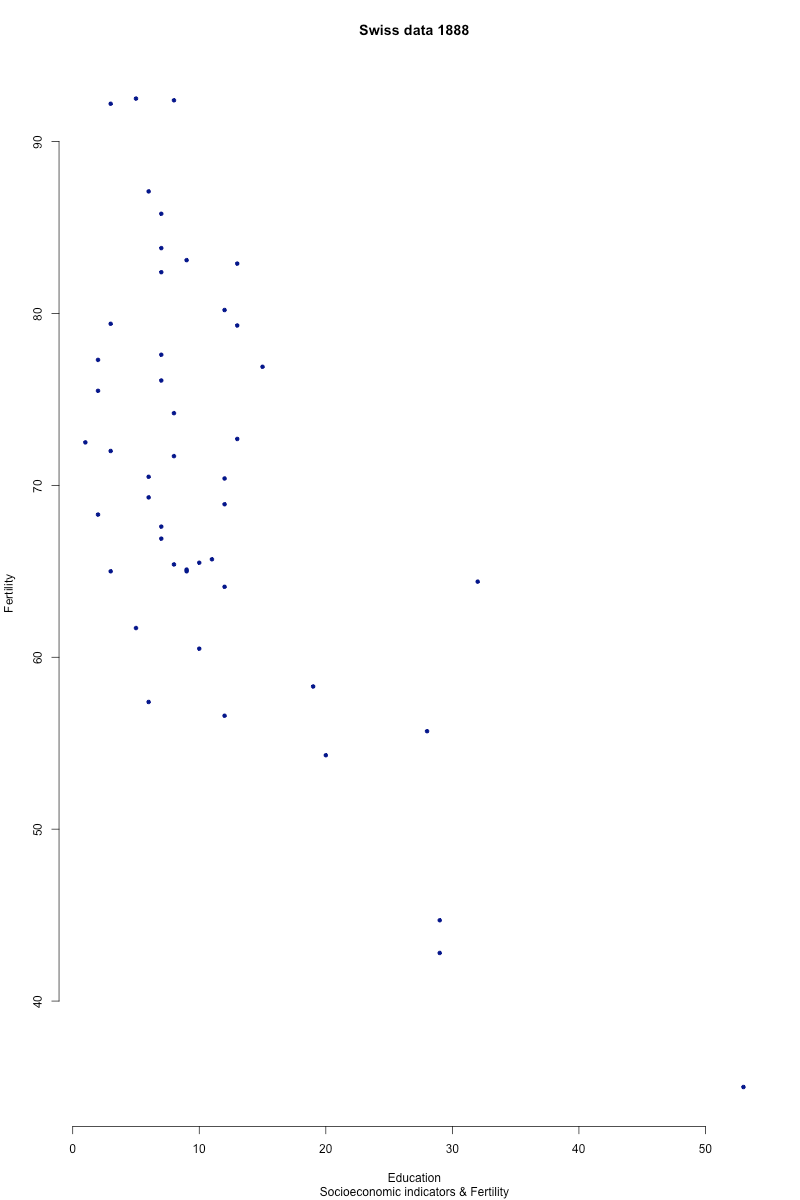
\includegraphics[width=0.5\textwidth]{/Users/lucas/Library/Mobile Documents/com~apple~CloudDocs/~~aa Study Materials/Grade 2 I/Learning/R for Data Science/Review of R/markdown/image/image-20231212160107785.png}

\textbf{Function usage:}

\begin{Shaded}
\begin{Highlighting}[]
\DocumentationTok{\#\# Default S3 method:}
\FunctionTok{plot}\NormalTok{(}
\NormalTok{  x, }
  \AttributeTok{y =} \ConstantTok{NULL}\NormalTok{, }
  \AttributeTok{type =} \StringTok{"p"}\NormalTok{, }
  \AttributeTok{xlim =} \ConstantTok{NULL}\NormalTok{, }\AttributeTok{ylim =} \ConstantTok{NULL}\NormalTok{,}
  \AttributeTok{log =} \StringTok{""}\NormalTok{, }
  \AttributeTok{main =} \ConstantTok{NULL}\NormalTok{, }\AttributeTok{sub =} \ConstantTok{NULL}\NormalTok{, }
  \AttributeTok{xlab =} \ConstantTok{NULL}\NormalTok{, }\AttributeTok{ylab =} \ConstantTok{NULL}\NormalTok{,}
  \AttributeTok{ann =} \FunctionTok{par}\NormalTok{(}\StringTok{"ann"}\NormalTok{), }\AttributeTok{axes =} \ConstantTok{TRUE}\NormalTok{, }\AttributeTok{frame.plot =}\NormalTok{ axes,}
  \AttributeTok{panel.first =} \ConstantTok{NULL}\NormalTok{, }\AttributeTok{panel.last =} \ConstantTok{NULL}\NormalTok{, }\AttributeTok{asp =} \ConstantTok{NA}\NormalTok{,}
  \AttributeTok{xgap.axis =} \ConstantTok{NA}\NormalTok{, }\AttributeTok{ygap.axis =} \ConstantTok{NA}\NormalTok{,}
\NormalTok{  ...}
\NormalTok{)}
\CommentTok{\# Default Parameters are listed.}
\end{Highlighting}
\end{Shaded}

\textbf{Arguments}

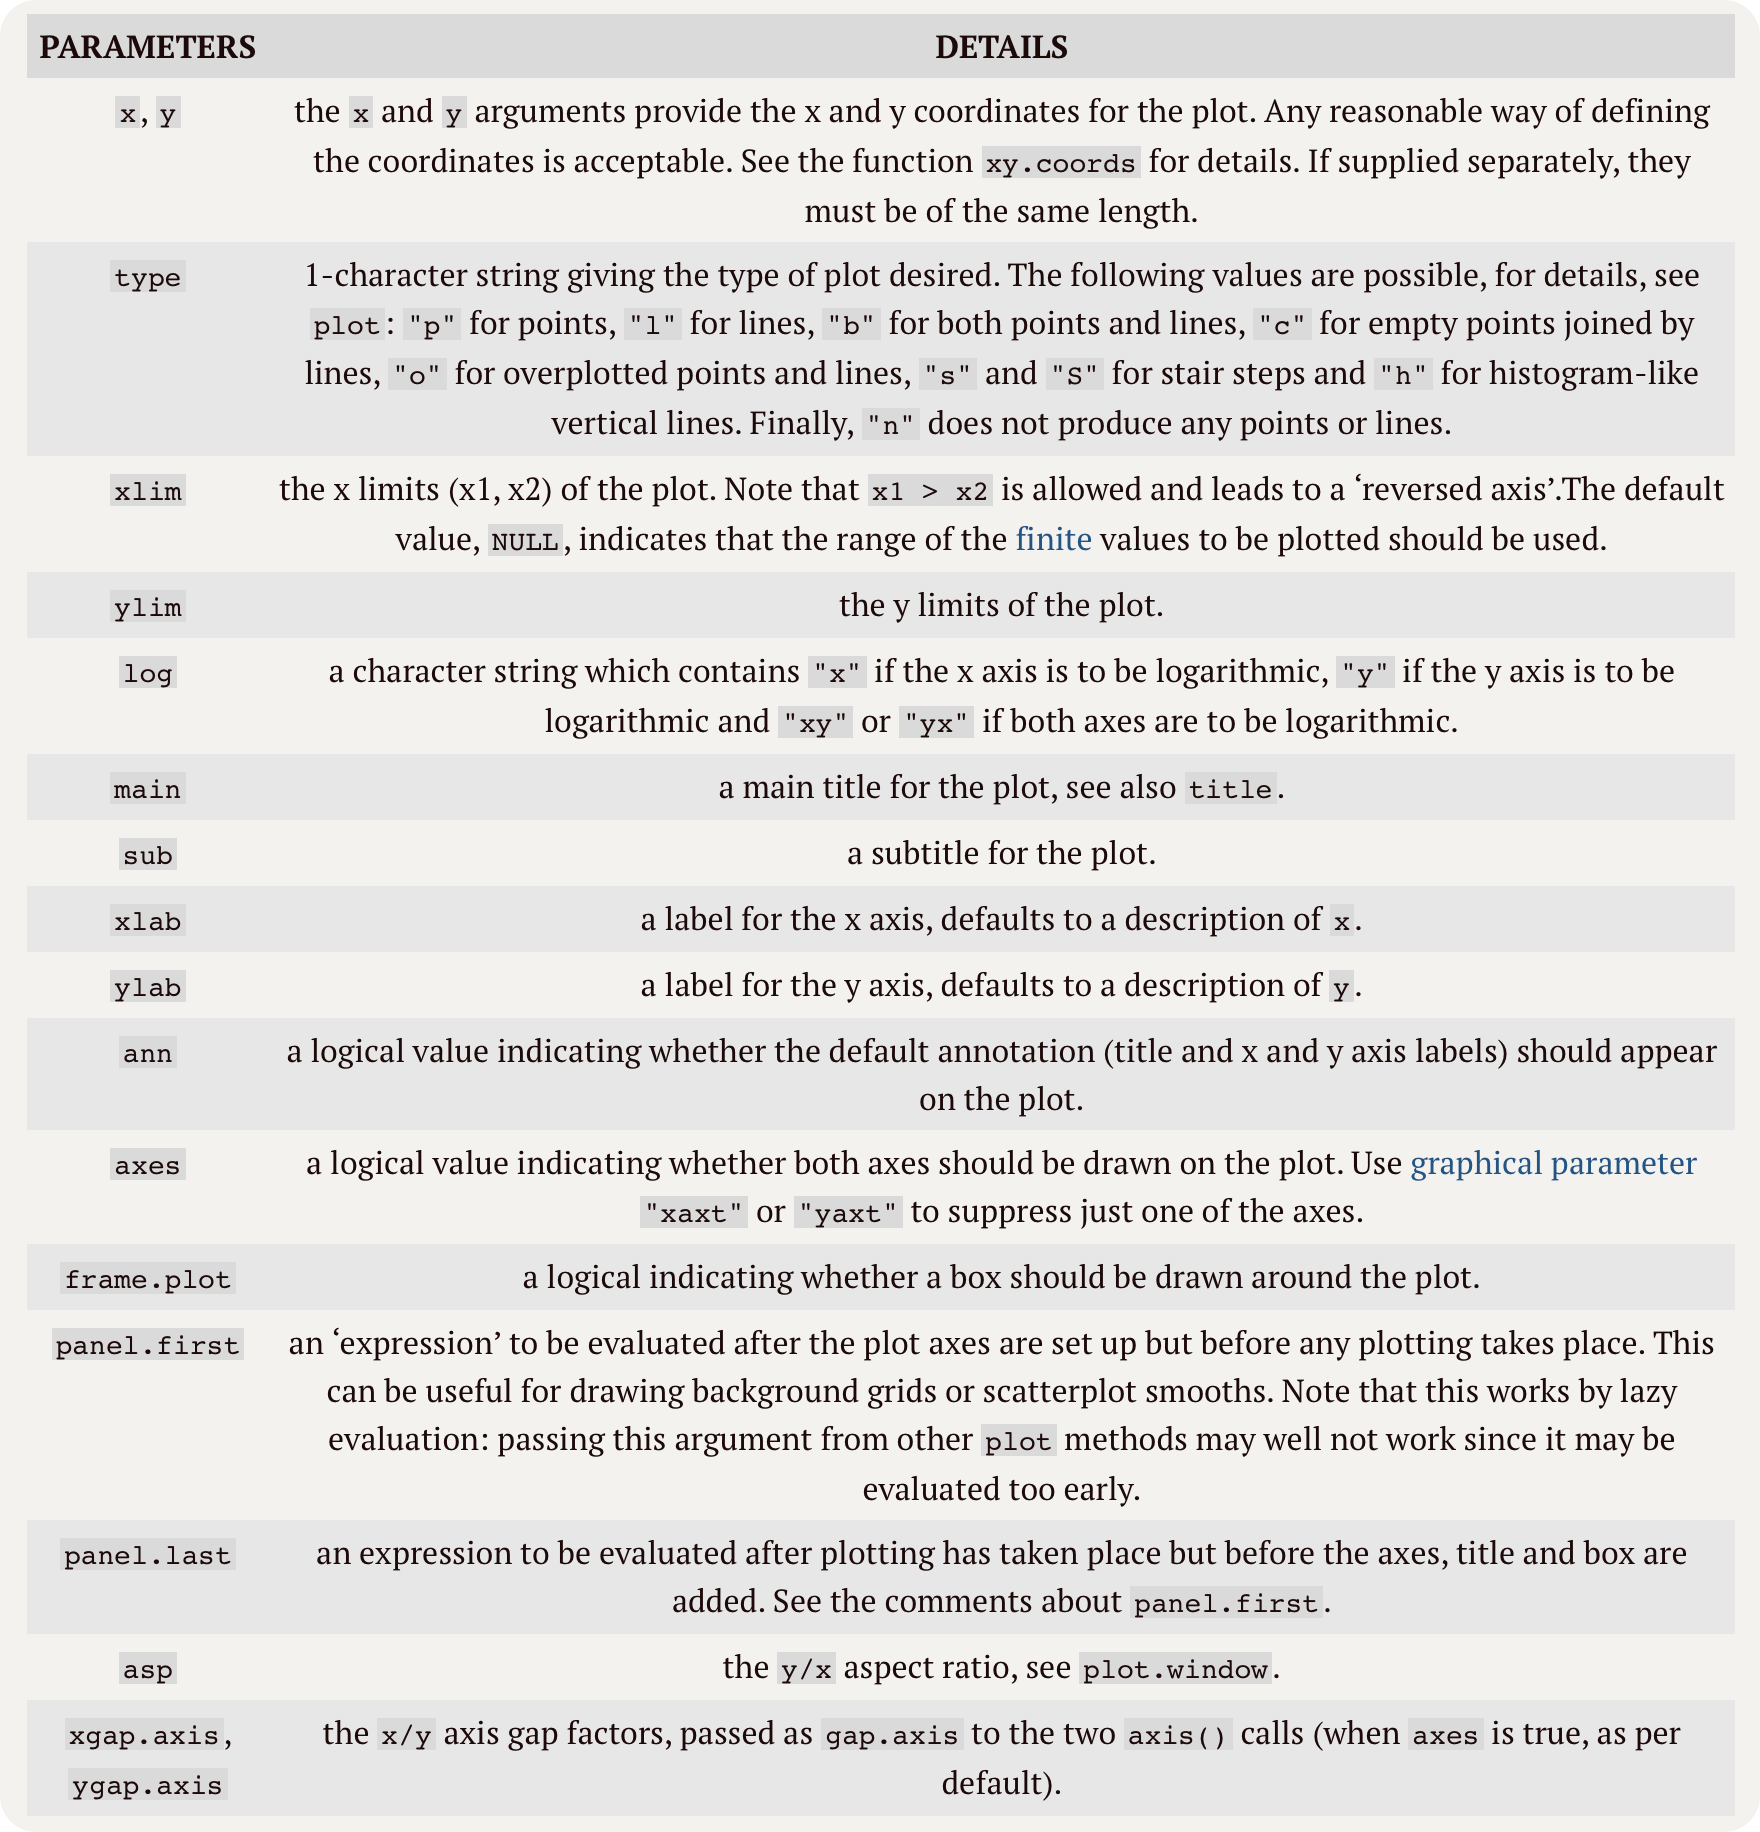
\includegraphics{/Users/lucas/Library/Mobile Documents/com~apple~CloudDocs/~~aa Study Materials/Grade 2 I/Learning/R for Data Science/Review of R/markdown/image/image-20231212194556462.png}

You can also use \texttt{ggplot} to draw the plot above:

\begin{Shaded}
\begin{Highlighting}[]
\FunctionTok{ggplot}\NormalTok{( }
\NormalTok{  swiss, }
  \FunctionTok{aes}\NormalTok{(}\AttributeTok{x =}\NormalTok{ Education, }\AttributeTok{y =}\NormalTok{ Fertility) }
\NormalTok{) }\SpecialCharTok{+} 
\FunctionTok{geom\_point}\NormalTok{() }\SpecialCharTok{+} 
\FunctionTok{scale\_x\_log10}\NormalTok{() }\SpecialCharTok{+} 
\FunctionTok{scale\_y\_log10}\NormalTok{() }\SpecialCharTok{+} 
\FunctionTok{xlab}\NormalTok{(}\StringTok{"Education"}\NormalTok{) }\SpecialCharTok{+} 
\FunctionTok{ylab}\NormalTok{(}\StringTok{"Fertility"}\NormalTok{) }\SpecialCharTok{+} 
\NormalTok{ggtitle }\StringTok{"Swiss data 1888"}\ErrorTok{)}
\end{Highlighting}
\end{Shaded}

\hypertarget{high-level-and-low-level}{%
\subsubsection{High-level and
low-level}\label{high-level-and-low-level}}

\begin{itemize}
\item
  \textbf{high level}: plotting functions create a new plot on the
  graphics device
\item
  \textbf{low level}: plotting functions add more information to an
  existing plot
\end{itemize}

\hypertarget{low-level-plots}{%
\paragraph{Low level plots}\label{low-level-plots}}

\begin{itemize}
\item
  \texttt{points} : dot plot
\item
  \texttt{lines} : line plot
\item
  \texttt{abline} : straightness
\item
  \texttt{polygon} : polygonal
\item
  \texttt{legend} : legend (of a map, etc)
\item
  \texttt{title} : caption
\item
  \texttt{axis} : axis
\end{itemize}

\hypertarget{high-level-plots}{%
\paragraph{High level plots}\label{high-level-plots}}

\begin{itemize}
\item
  \texttt{plot} : Generalized Graphing Functions
\item
  \texttt{pairs}
\item
  \texttt{coplot}
\item
  \texttt{qqnorm}
\item
  \texttt{hist}
\item
  \texttt{dotchart}
\item
  \texttt{image}
\item
  \texttt{contour}
\end{itemize}

\textbf{Notice}

You can force a high level function to be converted to low level with
the \texttt{add\ =\ TRUE} parameter (if available).

\hypertarget{graphics-related-parameters-system-functions}{%
\subsubsection{Graphics-related parameters (system
functions)}\label{graphics-related-parameters-system-functions}}

You can use \texttt{par()} to view all the parameters current grafical
device use.

\textbf{Remember to backup your default parameters before modyfy them.}

\hypertarget{ggplot2}{%
\subsection{\texorpdfstring{\texttt{ggplot2}}{ggplot2}}\label{ggplot2}}

You should know that

\begin{enumerate}
\def\labelenumi{\arabic{enumi}.}
\item
  \texttt{xy\ -axes} will automatically adjust based on the data you
  give;
\item
  \texttt{ggplot2} plotting results can be saved in variables and more
  layers can be added;
\item
  Layers using their own data need to be specified with
  \texttt{data\ =}, while global data is not. You can just specify it
  via \texttt{ggplot(data\ =\ data.frame(...))}.
\end{enumerate}

\hypertarget{some-basic-parameters-of-ggplot2}{%
\subsubsection{\texorpdfstring{Some basic parameters of
\texttt{ggplot2}}{Some basic parameters of ggplot2}}\label{some-basic-parameters-of-ggplot2}}

\begin{enumerate}
\def\labelenumi{\arabic{enumi}.}
\item
  \texttt{geom} - Layer

  \texttt{geom\_\textless{}name\_of\_the\_layer\textgreater{}}
\end{enumerate}

\begin{itemize}
\item
  \texttt{geom\_point} , \texttt{\textasciigrave{}\ geom\_line} : A
  point and line plot used to reveal the relationship between two sets
  of data;
\end{itemize}

\begin{itemize}
\item
  \texttt{geom\_smooth} : Often used in conjunction with
  \texttt{geom\_point} to reveal the trend of data.
\item
  \texttt{geom\_bar} : bar charts
\item
  \texttt{geom\_boxplot} : A box plot, used to compare N sets of data,
  revealing differences.
\item
  \texttt{geom\_path} : similar to \texttt{geom\_line} but can also draw
  other complex graphs
\item
  \texttt{geom\_histogram}, \texttt{geom\_density} : Distribution of
  data, can also be used to compare multiple groups.

  \ldots\ldots{}
\end{itemize}

\begin{enumerate}
\def\labelenumi{\arabic{enumi}.}
\item
  \texttt{scale} - Display Control

  \texttt{scale\_\textless{}property\_to\ \_control\textgreater{}\_\textless{}ways\_to\_control\textgreater{}}
\end{enumerate}

\begin{itemize}
\item
  \texttt{scale\_color\_...}

  \begin{itemize}
  \item
    \texttt{...\_gradient()}: use gradient colors for different numbers
    of variables and their colors.

    \begin{itemize}
    \item
      \texttt{...\_gradient2()}
    \item
      \texttt{...\_gradientn()}
    \end{itemize}
  \item
    \texttt{...\_brewer}: use default color palettes.
  \end{itemize}
\item
  \texttt{scale\_fill\_...}

  \begin{itemize}
  \item
    \texttt{colour} defines the colour with which a geom is
    \textbf{outlined} (the shape\textquotesingle s "stroke")
  \end{itemize}

  \begin{itemize}
  \item
    \texttt{fill}defines the colour with which a geom is \textbf{filled}
  \item
    Points generally only have a \texttt{colour} and \textbf{no fill}
  \item
    However, point shapes \textbf{21--25} that include \textbf{both} a
    colour and a fill.
  \end{itemize}
\item
  \texttt{scale\_shape\_...}
\item
  \texttt{scale\_size\_...}
\end{itemize}

\hypertarget{palettes-and-corresponding-functions-in-other-packages}{%
\paragraph{Palettes and corresponding functions in other
packages}\label{palettes-and-corresponding-functions-in-other-packages}}

\hypertarget{included-in-ggplot2}{%
\subparagraph{\texorpdfstring{Included in
\texttt{ggplot2}}{Included in ggplot2}}\label{included-in-ggplot2}}

\texttt{scale\_color\_hue}, \texttt{scale\_color\_manual},
\texttt{scale\_color\_grey}, \texttt{scale\_colour\_viridis\_d},
\texttt{scale\_color\_brewer} ...

\hypertarget{from-the-rcolorbrewer-package}{%
\subparagraph{\texorpdfstring{From the \texttt{RColorBrewer}
package}{From the RColorBrewer package}}\label{from-the-rcolorbrewer-package}}

\texttt{scale\_color\_brewer(palette\ =\ "\textless{}palette\ name\textgreater{}")}

\hypertarget{from-the-viridis-package}{%
\subparagraph{\texorpdfstring{From the \texttt{viridis}
package}{From the viridis package}}\label{from-the-viridis-package}}

\texttt{scale\_color\_viridis(discrete=TRUE,\ option="\textless{}palette\ name\textgreater{}")}

\hypertarget{other-packages-}{%
\subparagraph{Other packages ...}\label{other-packages-}}

\begin{itemize}
\item
  \texttt{paletteer} package: \texttt{scale\_color\_paletteer\_xx}
  functions
\item
  \texttt{ggsci} package
\item
  \texttt{ggsci}: You can use it in your SCI article.

  \begin{itemize}
  \item
    contents

    \texttt{scale\_color\_\textless{}journal\textgreater{}} 和
    \texttt{scale\_fill\_\textless{}journal\textgreater{}} functions and
    color palettes
  \end{itemize}
\end{itemize}

\begin{Shaded}
\begin{Highlighting}[]
\NormalTok{{-} supported journals}

\NormalTok{	* NPG \textasciigrave{}scale\_color\_npg()\textasciigrave{}, \textasciigrave{}scale\_fill\_npg()\textasciigrave{}}

\NormalTok{	* AAAS, NEJM, Lancet, JAMA ... }
\end{Highlighting}
\end{Shaded}

\begin{enumerate}
\def\labelenumi{\arabic{enumi}.}
\item
  \texttt{size}
\item
  \texttt{shape}
\end{enumerate}

\textbf{Question:}

Parameters like \texttt{size}, \texttt{colour} etc. can be inside or
outside \texttt{aes()}, what is the difference?

\textbf{Answer:}

In the internal case, the \textbf{size} is determined by the value of
the specified column, or the \textbf{number} of colors and shapes is
determined by the number of factors, and in the external case, the
\textbf{specified value} prevails.

\hypertarget{coordinate-system}{%
\subsubsection{Coordinate System}\label{coordinate-system}}

\begin{enumerate}
\def\labelenumi{\arabic{enumi}.}
\item
  Linear coordinate system
\end{enumerate}

\begin{itemize}
\item
  \texttt{coord\_cartesian()},

  You can use parameters like \texttt{xlim()} \& \texttt{ylim()} to
  \textbf{zoom in and out locally}.
\item
  \texttt{coord\_flip()},

  This parameter exchanges the \texttt{x} and \texttt{y} axes.
\item
  \texttt{coord\_fixed()}

  Draw plots in specific \textbf{aspect ratio}.
\end{itemize}

\begin{enumerate}
\def\labelenumi{\arabic{enumi}.}
\item
  Nonlinear coordinate system
\end{enumerate}

\begin{itemize}
\item
  \texttt{coord\_trans()}

  This parameter exchanges the \texttt{x} and \texttt{y} axes,
  \textbf{however}, it will plot the original figure, too.
\item
  \texttt{coord\_polar()}

  The default parameter is \texttt{coord\_polar(x)}.
\item
  \texttt{coord\_map()}

  World Map
\end{itemize}

\hypertarget{faceting}{%
\subsubsection{\texorpdfstring{\texttt{faceting}}{faceting}}\label{faceting}}

panel, strip, axis, tick, tick label, axis label\ldots{}

\begin{itemize}
\item
  \texttt{facet\_wrap()}

  Use to specify the number of rows, columns and orientation.

\begin{Shaded}
\begin{Highlighting}[]
\FunctionTok{facet\_wrap}\NormalTok{(}
\NormalTok{  facets,}
  \AttributeTok{nrow =} \ConstantTok{NULL}\NormalTok{,}
  \AttributeTok{ncol =} \ConstantTok{NULL}\NormalTok{,}
  \AttributeTok{scales =} \StringTok{"fixed"}\NormalTok{,}
  \AttributeTok{shrink =} \ConstantTok{TRUE}\NormalTok{,}
  \AttributeTok{labeller =} \StringTok{"label\_value"}\NormalTok{,}
  \AttributeTok{as.table =} \ConstantTok{TRUE}\NormalTok{,}
  \AttributeTok{switch =} \ConstantTok{NULL}\NormalTok{,}
  \AttributeTok{drop =} \ConstantTok{TRUE}\NormalTok{,}
  \AttributeTok{dir =} \StringTok{"h"}\NormalTok{,}
  \AttributeTok{strip.position =} \StringTok{"top"}
\NormalTok{)}

\CommentTok{\# Default parameters are listed.}
\end{Highlighting}
\end{Shaded}
\end{itemize}

\hypertarget{different-layouts}{%
\subsubsection{Different layouts}\label{different-layouts}}

Nothing to explain, for it's too intricate.

\hypertarget{formulas}{%
\subsection{Formulas}\label{formulas}}

\begin{quote}
Similar to \($\LaTeX$\)
\end{quote}

You can just type the formula as exactly what you type in \($\LaTeX$\),
and using \texttt{annotiate()} function to add it in your plot.

\textbf{Remember to attach the library \texttt{latex2exp}}

\begin{Shaded}
\begin{Highlighting}[]
\NormalTok{fig1 }\OtherTok{=}
\NormalTok{  fig1 }\SpecialCharTok{+}
  \FunctionTok{annotate}\NormalTok{(}
    \StringTok{"text"}\NormalTok{,}
    \AttributeTok{x =} \DecValTok{25}\NormalTok{,}
    \AttributeTok{y =} \DecValTok{15}\NormalTok{,}
    \AttributeTok{label =} \FunctionTok{paste0}\NormalTok{(}\StringTok{"y = "}\NormalTok{, eq, }\StringTok{"x + ("}\NormalTok{, intercept, }\StringTok{")}\SpecialCharTok{\textbackslash{}n}\StringTok{"}\NormalTok{,}\StringTok{"Shaded areas are confidence intervals."}\NormalTok{), }\CommentTok{\# nolint}
    \AttributeTok{family =} \StringTok{"Aptos Serif"}
\NormalTok{  )}
\end{Highlighting}
\end{Shaded}

\begin{Shaded}
\begin{Highlighting}[]
\NormalTok{... }\SpecialCharTok{+}
\FunctionTok{labs}\NormalTok{(}
    \AttributeTok{x =} \FunctionTok{TeX}\NormalTok{(}\StringTok{"Position of $P\_2/}\SpecialCharTok{\textbackslash{}\textbackslash{}}\StringTok{phi$"}\NormalTok{),}
    \AttributeTok{y =} \FunctionTok{TeX}\NormalTok{(}\StringTok{"Light Intensity/$10\^{}\{{-}7\}$A"}\NormalTok{),}
    \AttributeTok{title =} \FunctionTok{TeX}\NormalTok{(}\StringTok{"Intensity of Light with Different $}\SpecialCharTok{\textbackslash{}\textbackslash{}}\StringTok{phi$"}\NormalTok{)}
\NormalTok{  )}
\end{Highlighting}
\end{Shaded}

\textbf{Something about \texttt{hjust} and \texttt{vjust}}

\begin{Shaded}
\begin{Highlighting}[]
\NormalTok{td }\OtherTok{=} \FunctionTok{expand.grid}\NormalTok{(}
    \AttributeTok{hjust=}\FunctionTok{c}\NormalTok{(}\DecValTok{0}\NormalTok{, }\FloatTok{0.5}\NormalTok{, }\DecValTok{1}\NormalTok{),}
    \AttributeTok{vjust=}\FunctionTok{c}\NormalTok{(}\DecValTok{0}\NormalTok{, }\FloatTok{0.5}\NormalTok{, }\DecValTok{1}\NormalTok{),}
    \AttributeTok{angle=}\FunctionTok{c}\NormalTok{(}\DecValTok{0}\NormalTok{, }\DecValTok{45}\NormalTok{, }\DecValTok{90}\NormalTok{),}
    \AttributeTok{text=}\StringTok{"text"}
\NormalTok{)}

\FunctionTok{ggplot}\NormalTok{(td, }\FunctionTok{aes}\NormalTok{(}\AttributeTok{x=}\NormalTok{hjust, }\AttributeTok{y=}\NormalTok{vjust)) }\SpecialCharTok{+} 
    \FunctionTok{geom\_point}\NormalTok{() }\SpecialCharTok{+}
    \FunctionTok{geom\_text}\NormalTok{(}\FunctionTok{aes}\NormalTok{(}\AttributeTok{label=}\NormalTok{text, }\AttributeTok{angle=}\NormalTok{angle, }\AttributeTok{hjust=}\NormalTok{hjust, }\AttributeTok{vjust=}\NormalTok{vjust)) }\SpecialCharTok{+} 
    \FunctionTok{facet\_grid}\NormalTok{(}\SpecialCharTok{\textasciitilde{}}\NormalTok{angle) }\SpecialCharTok{+}
    \FunctionTok{scale\_x\_continuous}\NormalTok{(}\AttributeTok{breaks=}\FunctionTok{c}\NormalTok{(}\DecValTok{0}\NormalTok{, }\FloatTok{0.5}\NormalTok{, }\DecValTok{1}\NormalTok{), }\AttributeTok{expand=}\FunctionTok{c}\NormalTok{(}\DecValTok{0}\NormalTok{, }\FloatTok{0.2}\NormalTok{)) }\SpecialCharTok{+}
    \FunctionTok{scale\_y\_continuous}\NormalTok{(}\AttributeTok{breaks=}\FunctionTok{c}\NormalTok{(}\DecValTok{0}\NormalTok{, }\FloatTok{0.5}\NormalTok{, }\DecValTok{1}\NormalTok{), }\AttributeTok{expand=}\FunctionTok{c}\NormalTok{(}\DecValTok{0}\NormalTok{, }\FloatTok{0.2}\NormalTok{))}
\end{Highlighting}
\end{Shaded}

\textbf{You should always remember, the first step you want to draw a
plot is to calculate the data.}

\begin{center}\rule{0.5\linewidth}{0.5pt}\end{center}

\hypertarget{r-for-bioinformatics-data-summarisation-and-statistics}{%
\section{R for bioinformatics, data summarisation and
statistics}\label{r-for-bioinformatics-data-summarisation-and-statistics}}

\begin{quote}
Talk 10
\end{quote}

\hypertarget{toc-2}{%
\subsection{TOC}\label{toc-2}}

\begin{itemize}
\item
  Data summarisation functions (vector data)

  \begin{itemize}
  \item
    median, mean, sd, quantile, summary
  \end{itemize}
\item
  Graphical data summarisation (two-D data/ tibble/ table)

  \begin{itemize}
  \item
    dot plot
  \item
    smooth
  \item
    linear regression
  \item
    correlation \& variance explained
  \item
    groupping \& bar/ box/ plots
  \end{itemize}
\item
  statistics

  \begin{itemize}
  \item
    parametric tests

    \begin{itemize}
    \item
      t-test
    \item
      one way ANNOVA
    \item
      two way ANNOVA
    \item
      linear regression
    \item
      model / prediction / coefficients
    \end{itemize}
  \item
    non-parametric comparison
  \end{itemize}
\end{itemize}

\hypertarget{vector-summarization}{%
\subsection{Vector Summarization}\label{vector-summarization}}

\hypertarget{describe-normal-distribution}{%
\subsubsection{Describe Normal
Distribution}\label{describe-normal-distribution}}

You can use \texttt{mean} and \texttt{sd} to describe normal
distributions.

\begin{itemize}
\item
  It\textquotesingle s symmetrical.
\item
  Mean and median are the same.
\item
  Most common values are near the mean; less common values are farther
  from it.
\item
  Standard deviation marks the distance from the mean to the inflection
  point.
\end{itemize}

\hypertarget{functions-to-generate-random-normal-distrubions}{%
\subsubsection{Functions to generate random normal
distrubions}\label{functions-to-generate-random-normal-distrubions}}

\begin{Shaded}
\begin{Highlighting}[]
\FunctionTok{qnorm}\NormalTok{()}
\FunctionTok{pnorm}\NormalTok{()}
\FunctionTok{dnorm}\NormalTok{()}
\end{Highlighting}
\end{Shaded}

\hypertarget{other-regular-distributions}{%
\subsubsection{Other regular
distributions}\label{other-regular-distributions}}

\begin{enumerate}
\def\labelenumi{\arabic{enumi}.}
\item
  Uniform Distributions

\begin{Shaded}
\begin{Highlighting}[]
\FunctionTok{dunif}\NormalTok{(x, }\AttributeTok{min =} \DecValTok{0}\NormalTok{, }\AttributeTok{max =} \DecValTok{1}\NormalTok{, }\AttributeTok{log =} \ConstantTok{FALSE}\NormalTok{)}
\FunctionTok{punif}\NormalTok{(q, }\AttributeTok{min =} \DecValTok{0}\NormalTok{, }\AttributeTok{max =} \DecValTok{1}\NormalTok{, }\AttributeTok{lower.tail =} \ConstantTok{TRUE}\NormalTok{, }\AttributeTok{log.p =} \ConstantTok{FALSE}\NormalTok{)}
\FunctionTok{qunif}\NormalTok{(p, }\AttributeTok{min =} \DecValTok{0}\NormalTok{, }\AttributeTok{max =} \DecValTok{1}\NormalTok{, }\AttributeTok{lower.tail =} \ConstantTok{TRUE}\NormalTok{, }\AttributeTok{log.p =} \ConstantTok{FALSE}\NormalTok{)}
\FunctionTok{runif}\NormalTok{(n, }\AttributeTok{min =} \DecValTok{0}\NormalTok{, }\AttributeTok{max =} \DecValTok{1}\NormalTok{)}
\end{Highlighting}
\end{Shaded}
\item
  Non-parametric Distributions

  Here's an example:

\begin{Shaded}
\begin{Highlighting}[]
\NormalTok{bi }\OtherTok{=}
	\FunctionTok{c}\NormalTok{(}\DecValTok{7}\NormalTok{, }\DecValTok{3}\NormalTok{, }\DecValTok{2}\NormalTok{, }\DecValTok{1}\NormalTok{, }\DecValTok{7}\NormalTok{, }
    \DecValTok{3}\NormalTok{, }\DecValTok{4}\NormalTok{, }\DecValTok{5}\NormalTok{, }\DecValTok{7}\NormalTok{, }\DecValTok{6}\NormalTok{,}
    \DecValTok{2}\NormalTok{, }\DecValTok{2}\NormalTok{, }\DecValTok{1}\NormalTok{, }\DecValTok{3}\NormalTok{, }\DecValTok{7}\NormalTok{, }
    \DecValTok{2}\NormalTok{, }\DecValTok{6}\NormalTok{, }\DecValTok{8}\NormalTok{, }\DecValTok{2}\NormalTok{, }\DecValTok{7}\NormalTok{,}
    \DecValTok{2}\NormalTok{, }\DecValTok{2}\NormalTok{, }\DecValTok{1}\NormalTok{, }\DecValTok{3}\NormalTok{, }\DecValTok{5}\NormalTok{, }
    \DecValTok{8}\NormalTok{, }\DecValTok{2}\NormalTok{, }\DecValTok{6}\NormalTok{, }\DecValTok{7}\NormalTok{, }\DecValTok{8}\NormalTok{, }
    \DecValTok{6}\NormalTok{, }\DecValTok{2}\NormalTok{, }\DecValTok{8}\NormalTok{, }\DecValTok{7}\NormalTok{, }\DecValTok{9}\NormalTok{, }
    \DecValTok{2}\NormalTok{, }\DecValTok{7}\NormalTok{, }\DecValTok{5}\NormalTok{, }\DecValTok{1}\NormalTok{, }\DecValTok{8}\NormalTok{, }
    \DecValTok{8}\NormalTok{, }\DecValTok{2}\NormalTok{, }\DecValTok{3}\NormalTok{, }\DecValTok{7}\NormalTok{, }\DecValTok{3}
\NormalTok{   )}
\FunctionTok{ggplot}\NormalTok{( }
  \FunctionTok{data.frame}\NormalTok{(}\AttributeTok{dat =}\NormalTok{ bi),}
  \FunctionTok{aes}\NormalTok{(dat)) }\SpecialCharTok{+} 
\FunctionTok{geom\_density}\NormalTok{()}
\end{Highlighting}
\end{Shaded}
\end{enumerate}

\hypertarget{quantitative-descriptive-data}{%
\subsubsection{Quantitative descriptive
data}\label{quantitative-descriptive-data}}

\begin{itemize}
\item
  \textbf{mean}: aka average, is the sum of all of the numbers in the
  data set divided by the size of the data set;
\item
  \textbf{median}: The median is the value that is in the middle when
  the numbers in a data set are sorted in increasing order;
\item
  \textbf{sd}: standard deviation;
\item
  \textbf{var}: measures how far a set of numbers are spread out;
\item
  \textbf{range}: range of values.
\end{itemize}

\hypertarget{quantitative-descriptive-function}{%
\subsubsection{Quantitative descriptive
function}\label{quantitative-descriptive-function}}

Besides the function with the same name of the data above,
\texttt{quantile} and \texttt{summary} are two quantitative descriptive
functions.

\textbf{This chapter contains lots of functions and their usage, to know
more, you can see them in the official R documentation, I only explane
the things above here.}

\hypertarget{statistics}{%
\subsection{Statistics}\label{statistics}}

\hypertarget{parametric-tests}{%
\subsubsection{Parametric tests}\label{parametric-tests}}

\hypertarget{t-test}{%
\paragraph{\texorpdfstring{\texttt{t-test}}{t-test}}\label{t-test}}

Detect whether the distribution is consistent with expectations; e.g.,
whether the number of steps per day for boys is significantly different
from 10,000.

The test assesses whether the means of two samples are significantly
different from each other, assuming that the samples are normally
distributed and have approximately equal variances.

There are different types of t-tests in R, depending on the nature of
the comparison:

\begin{enumerate}
\def\labelenumi{\arabic{enumi}.}
\item
  \textbf{One-Sample t-test:}

  Used to determine if the mean of a single sample differs significantly
  from a known or hypothesized population mean.

  Example:

\begin{Shaded}
\begin{Highlighting}[]
\NormalTok{RCopy code}
\NormalTok{\# One{-}sample t{-}test example}
\NormalTok{sample\_data = c(17, 21, 19, 23, 20, 18, 22)}
\NormalTok{t.test(sample\_data, mu = 20)}
\end{Highlighting}
\end{Shaded}

  This code performs a one-sample t-test on \texttt{sample\_data} to
  test if its mean differs significantly from 20.
\item
  \textbf{Independent Samples t-test (or Two-Sample t-test):}

  Compares the means of two independent groups to determine if they are
  significantly different from each other.

  Example:

\begin{Shaded}
\begin{Highlighting}[]
\NormalTok{RCopy code}
\NormalTok{\# Independent samples t{-}test example}
\NormalTok{group1 = c(23, 25, 28, 22, 20)}
\NormalTok{group2 = c(18, 21, 24, 19, 17)}
\NormalTok{t.test(group1, group2)}
\end{Highlighting}
\end{Shaded}

  This code performs an independent samples t-test on \texttt{group1}
  and \texttt{group2} to test if their means are significantly
  different.
\item
  \textbf{Paired t-test:}

  Compares the means of two related groups (e.g., before and after
  measurements) to determine if they are significantly different.

  Example:

\begin{Shaded}
\begin{Highlighting}[]
\NormalTok{RCopy code}
\NormalTok{\# Paired t{-}test example}
\NormalTok{before = c(32, 28, 30, 29, 31)}
\NormalTok{after = c(30, 25, 28, 27, 29)}
\NormalTok{t.test(before, after, paired = TRUE)}
\end{Highlighting}
\end{Shaded}

  This code performs a paired t-test on \texttt{before} and
  \texttt{after} to test if there\textquotesingle s a significant
  difference.
\end{enumerate}

The \texttt{t.test()} function in R is used to conduct these t-tests. It
returns a test statistic (t-value), degrees of freedom, p-value, and
confidence interval, providing insights into whether the difference
observed is statistically significant.

It\textquotesingle s important to ensure that the assumptions of
normality and equal variances are met for reliable results when
performing t-tests in R. If the assumptions are violated, alternative
tests or data transformations might be more appropriate.

\hypertarget{one-way-annova}{%
\paragraph{One-way ANNOVA}\label{one-way-annova}}

In R, the one-way analysis of variance (ANOVA) is used to test for
significant differences between the means of three or more independent
(unrelated) groups. It assesses whether the means of these groups are
significantly different from each other.

The one-way ANOVA assumes that the data meet certain assumptions,
including:

\begin{itemize}
\item
  Normality: Each group should follow a normal distribution.
\item
  Homogeneity of variances: The variances within each group should be
  approximately equal.
\item
  Independence: The observations within each group should be independent
  of each other.
\end{itemize}

Here\textquotesingle s an example of performing a one-way ANOVA in R:

\begin{Shaded}
\begin{Highlighting}[]
\CommentTok{\# Example of one{-}way ANOVA}
\NormalTok{group1 }\OtherTok{=} \FunctionTok{c}\NormalTok{(}\DecValTok{15}\NormalTok{, }\DecValTok{20}\NormalTok{, }\DecValTok{25}\NormalTok{, }\DecValTok{30}\NormalTok{, }\DecValTok{35}\NormalTok{)}
\NormalTok{group2 }\OtherTok{=} \FunctionTok{c}\NormalTok{(}\DecValTok{10}\NormalTok{, }\DecValTok{18}\NormalTok{, }\DecValTok{25}\NormalTok{, }\DecValTok{32}\NormalTok{, }\DecValTok{40}\NormalTok{)}
\NormalTok{group3 }\OtherTok{=} \FunctionTok{c}\NormalTok{(}\DecValTok{12}\NormalTok{, }\DecValTok{22}\NormalTok{, }\DecValTok{28}\NormalTok{, }\DecValTok{32}\NormalTok{, }\DecValTok{38}\NormalTok{)}

\CommentTok{\# Combining data into a data frame}
\NormalTok{my\_data }\OtherTok{=} \FunctionTok{data.frame}\NormalTok{(}
  \AttributeTok{Values =} \FunctionTok{c}\NormalTok{(group1, group2, group3),}
  \AttributeTok{Group =} \FunctionTok{factor}\NormalTok{(}\FunctionTok{rep}\NormalTok{(}\DecValTok{1}\SpecialCharTok{:}\DecValTok{3}\NormalTok{, }\AttributeTok{each =} \DecValTok{5}\NormalTok{))  }\CommentTok{\# Creating a factor for groups}
\NormalTok{)}

\CommentTok{\# Performing one{-}way ANOVA}
\NormalTok{result\_anova }\OtherTok{=} \FunctionTok{aov}\NormalTok{(Values }\SpecialCharTok{\textasciitilde{}}\NormalTok{ Group, }\AttributeTok{data =}\NormalTok{ my\_data)}
\FunctionTok{summary}\NormalTok{(result\_anova)}
\end{Highlighting}
\end{Shaded}

Explanation of the code:

\begin{enumerate}
\def\labelenumi{\arabic{enumi}.}
\item
  The data for three groups (\texttt{group1}, \texttt{group2},
  \texttt{group3}) are created.
\item
  The data are combined into a data frame (\texttt{my\_data}) where the
  \texttt{Values} column contains the measurements and the
  \texttt{Group} column represents the group labels as a factor.
\item
  The \texttt{aov()} function is used to perform the one-way ANOVA,
  specifying the formula \texttt{Values\ \textasciitilde{}\ Group},
  indicating that \texttt{Values} is the dependent variable and
  \texttt{Group} is the independent variable.
\item
  \texttt{summary(result\_anova)} provides the ANOVA table with the
  F-statistic, degrees of freedom, p-value, and other relevant
  statistics.
\end{enumerate}

The output from \texttt{summary(result\_anova)} will include information
such as the F-statistic, degrees of freedom, p-value, and within-group
variability, allowing you to determine if there are significant
differences between the means of the groups.

If the p-value is less than a chosen significance level (commonly 0.05),
it suggests that there are significant differences among the means of
the groups. Additionally, post-hoc tests like Tukey\textquotesingle s
HSD test or pairwise t-tests can be performed to identify which specific
groups differ significantly from each other after obtaining a
significant result in the ANOVA.

\hypertarget{two-way-annova}{%
\paragraph{Two-way ANNOVA}\label{two-way-annova}}

A two-way analysis of variance (ANOVA) in R is used to examine the
interaction effects between two categorical independent variables
(factors) on a continuous dependent variable.

Here\textquotesingle s an example:

\begin{Shaded}
\begin{Highlighting}[]
\CommentTok{\# Example of two{-}way ANOVA}
\CommentTok{\# Assume we have a dataset with \textquotesingle{}Treatment\textquotesingle{}, \textquotesingle{}Gender\textquotesingle{}, and \textquotesingle{}Response\textquotesingle{} variables}

\CommentTok{\# Creating sample data}
\FunctionTok{set.seed}\NormalTok{(}\DecValTok{123}\NormalTok{)}
\NormalTok{Treatment }\OtherTok{=} \FunctionTok{rep}\NormalTok{(}\FunctionTok{c}\NormalTok{(}\StringTok{"A"}\NormalTok{, }\StringTok{"B"}\NormalTok{, }\StringTok{"C"}\NormalTok{), }\AttributeTok{each =} \DecValTok{20}\NormalTok{)}
\NormalTok{Gender }\OtherTok{=} \FunctionTok{rep}\NormalTok{(}\FunctionTok{c}\NormalTok{(}\StringTok{"Male"}\NormalTok{, }\StringTok{"Female"}\NormalTok{), }\AttributeTok{times =} \DecValTok{30}\NormalTok{)}
\NormalTok{Response }\OtherTok{=} \FunctionTok{rnorm}\NormalTok{(}\DecValTok{60}\NormalTok{, }\AttributeTok{mean =} \FunctionTok{c}\NormalTok{(}\DecValTok{50}\NormalTok{, }\DecValTok{60}\NormalTok{, }\DecValTok{70}\NormalTok{), }\AttributeTok{sd =} \DecValTok{10}\NormalTok{)}

\CommentTok{\# Combining data into a data frame}
\NormalTok{my\_data }\OtherTok{=} \FunctionTok{data.frame}\NormalTok{(Treatment, Gender, Response)}

\CommentTok{\# Performing two{-}way ANOVA}
\NormalTok{result\_anova }\OtherTok{=} \FunctionTok{aov}\NormalTok{(Response }\SpecialCharTok{\textasciitilde{}}\NormalTok{ Treatment }\SpecialCharTok{+}\NormalTok{ Gender }\SpecialCharTok{+}\NormalTok{ Treatment}\SpecialCharTok{:}\NormalTok{Gender, }\AttributeTok{data =}\NormalTok{ my\_data)}
\FunctionTok{summary}\NormalTok{(result\_anova)}
\end{Highlighting}
\end{Shaded}

Explanation of the code:

\begin{enumerate}
\def\labelenumi{\arabic{enumi}.}
\item
  Sample data is created with three variables: \texttt{Treatment},
  \texttt{Gender}, and \texttt{Response}.
\item
  The data are combined into a data frame (\texttt{my\_data}), where
  \texttt{Treatment} and \texttt{Gender} are categorical factors, and
  \texttt{Response} is the continuous dependent variable.
\item
  The \texttt{aov()} function performs the two-way ANOVA. The formula
  \texttt{Response\ \textasciitilde{}\ Treatment\ +\ Gender\ +\ Treatment:Gender}
  specifies the main effects of \texttt{Treatment} and \texttt{Gender},
  as well as their interaction effect.
\item
  \texttt{summary(result\_anova)} provides the ANOVA table with
  F-statistics, degrees of freedom, p-values, and other statistics for
  each factor and their interaction.
\end{enumerate}

The output from \texttt{summary(result\_anova)} will include information
about the main effects of \texttt{Treatment} and \texttt{Gender}, as
well as the interaction effect between them. It allows you to determine
if there are significant effects of each factor independently and
whether their interaction significantly influences the \texttt{Response}
variable.

The interpretation of a two-way ANOVA involves analyzing the p-values
associated with each factor and their interaction. Significant p-values
indicate that the corresponding factor or interaction has a significant
effect on the dependent variable. Additionally, post-hoc tests or
further analyses can be conducted to explore specific comparisons
between groups or factors after obtaining significant results in the
ANOVA.

\hypertarget{linear-regression}{%
\paragraph{Linear Regression}\label{linear-regression}}

Linear regression is a statistical method used to model the relationship
between a dependent variable and one or more independent variables by
fitting a linear equation to observed data. In R, linear regression can
be performed using the \texttt{lm()} function, which stands for "linear
model."

Here\textquotesingle s an example:

\begin{Shaded}
\begin{Highlighting}[]
\CommentTok{\# Example of simple linear regression}
\CommentTok{\# Suppose we have a dataset with \textquotesingle{}x\textquotesingle{} as the independent variable and \textquotesingle{}y\textquotesingle{} as the dependent variable}

\CommentTok{\# Creating sample data}
\FunctionTok{set.seed}\NormalTok{(}\DecValTok{123}\NormalTok{)}
\NormalTok{x }\OtherTok{=} \DecValTok{1}\SpecialCharTok{:}\DecValTok{50}
\NormalTok{y }\OtherTok{=} \DecValTok{2} \SpecialCharTok{*}\NormalTok{ x }\SpecialCharTok{+} \FunctionTok{rnorm}\NormalTok{(}\DecValTok{50}\NormalTok{, }\AttributeTok{mean =} \DecValTok{0}\NormalTok{, }\AttributeTok{sd =} \DecValTok{5}\NormalTok{)  }\CommentTok{\# Generating \textquotesingle{}y\textquotesingle{} as a linear function of \textquotesingle{}x\textquotesingle{} with some noise}

\CommentTok{\# Creating a data frame}
\NormalTok{my\_data }\OtherTok{=} \FunctionTok{data.frame}\NormalTok{(x, y)}

\CommentTok{\# Performing linear regression}
\NormalTok{model }\OtherTok{=} \FunctionTok{lm}\NormalTok{(y }\SpecialCharTok{\textasciitilde{}}\NormalTok{ x, }\AttributeTok{data =}\NormalTok{ my\_data)}
\FunctionTok{summary}\NormalTok{(model)}
\end{Highlighting}
\end{Shaded}

Explanation of the code:

\begin{enumerate}
\def\labelenumi{\arabic{enumi}.}
\item
  Sample data is generated with an independent variable \texttt{x} and a
  dependent variable \texttt{y}. In this example, \texttt{y} is
  generated as a linear function of \texttt{x} with some added noise
  using \texttt{rnorm()} to simulate real-world variability.
\item
  The data are combined into a data frame \texttt{my\_data}.
\item
  The \texttt{lm()} function fits a linear regression model where
  \texttt{y} is the dependent variable and \texttt{x} is the independent
  variable (\texttt{y\ \textasciitilde{}\ x}). The argument
  \texttt{data\ =\ my\_data} specifies the data frame containing the
  variables.
\item
  \texttt{summary(model)} provides a summary of the linear regression
  model, including coefficients, standard errors, t-values, p-values,
  R-squared, and other statistics.
\end{enumerate}

Interpreting the output from \texttt{summary(model)}:

\begin{itemize}
\item
  The coefficients section shows the estimated coefficients for the
  intercept and the slope of the regression line (\texttt{Intercept} and
  \texttt{x}).
\item
  The p-values associated with the coefficients indicate the
  significance of each variable in predicting the dependent variable.
  Lower p-values suggest stronger evidence against the null hypothesis
  of no effect.
\item
  The R-squared value represents the proportion of variance in the
  dependent variable explained by the independent variable(s). Higher
  R-squared values indicate a better fit of the model to the data.
\end{itemize}

Linear regression in R can also be extended to multiple linear
regression by including multiple independent variables in the model
(\texttt{y\ \textasciitilde{}\ x1\ +\ x2\ +\ ...}). Additionally,
diagnostic plots and further analyses can be performed to assess model
assumptions and goodness of fit.

\hypertarget{model--prediction--coefficients}{%
\paragraph{Model / Prediction /
Coefficients}\label{model--prediction--coefficients}}

Certainly! In linear regression, the model equation is expressed as:

\([ y = \beta_0 + \beta_1 \cdot x_1 + \beta_2 \cdot x_2 + \ldots + \beta_n \cdot x_n + \epsilon ]\)

Where:

\begin{itemize}
\item
  ( \(y\) ) is the dependent variable.
\item
  (\( x_1, x_2, \ldots, x_n\) ) are the independent variables.
\item
  ( \(\beta_0\) ) is the intercept (constant term).
\item
  ( \(\beta_1, \beta_2, \ldots, \beta_n\) ) are the coefficients (slope
  parameters) that represent the change in ( \(y\) ) associated with a
  one-unit change in the corresponding ( \(x\) ) variable, assuming all
  other variables remain constant.
\item
  ( \(\epsilon\) ) represents the error term.
\end{itemize}

In R, after fitting a linear regression model using \texttt{lm()}:

\begin{Shaded}
\begin{Highlighting}[]
\CommentTok{\# Assuming \textquotesingle{}model\textquotesingle{} is the linear regression model obtained previously}
\FunctionTok{summary}\NormalTok{(model)}
\end{Highlighting}
\end{Shaded}

The output from \texttt{summary(model)} provides information including:

\begin{itemize}
\item
  \textbf{Coefficients:} This section displays the estimated
  coefficients (\texttt{Estimate}) for each independent variable,
  including the intercept. These coefficients represent the estimated
  change in the dependent variable for a one-unit change in the
  corresponding independent variable, holding other variables constant.
\item
  \textbf{Residuals:} The residuals represent the differences between
  the observed and predicted values of the dependent variable. These are
  used to assess the goodness of fit of the model.
\item
  \textbf{R-squared:} Indicates the proportion of variance in the
  dependent variable explained by the independent variables. Higher
  values indicate a better fit of the model to the data.
\end{itemize}

After obtaining the coefficients from the model, predictions can be made
using new or existing data:

\begin{Shaded}
\begin{Highlighting}[]
\CommentTok{\# Assuming \textquotesingle{}new\_data\textquotesingle{} contains the new data for prediction}
\NormalTok{predicted\_values }\OtherTok{=} \FunctionTok{predict}\NormalTok{(model, }\AttributeTok{newdata =}\NormalTok{ new\_data)}
\end{Highlighting}
\end{Shaded}

Replace \texttt{new\_data} with the data for which you want to make
predictions. The \texttt{predict()} function uses the coefficients from
the model to generate predicted values of the dependent variable based
on the independent variables in the new data.

The coefficients obtained from the linear regression model
(\texttt{model\$coefficients}) represent the slopes of the regression
line and the intercept, which are crucial for predicting new values and
understanding the relationships between variables in the model.

\hypertarget{non-parametric-comparison}{%
\subsubsection{Non-parametric
Comparison}\label{non-parametric-comparison}}

Non-parametric methods are statistical techniques used when the
assumptions of normality, homogeneity of variances, or linearity
required by parametric methods are violated or not met by the data.
These methods do not rely on specific population distribution
assumptions and are useful for analyzing data that might not follow a
normal distribution.

Here are some commonly used non-parametric methods for comparison in R:

\begin{enumerate}
\def\labelenumi{\arabic{enumi}.}
\item
  \textbf{Mann-Whitney U Test (Wilcoxon Rank-Sum Test):}

  Used to compare two independent groups when the assumptions of t-tests
  are not met.

  Example:

\begin{Shaded}
\begin{Highlighting}[]
\CommentTok{\# Assuming \textquotesingle{}group1\textquotesingle{} and \textquotesingle{}group2\textquotesingle{} are vectors of numeric data}
\FunctionTok{wilcox.test}\NormalTok{(group1, group2)}
\end{Highlighting}
\end{Shaded}
\item
  \textbf{Kruskal-Wallis Test:}

  An extension of the Mann-Whitney U test for comparing more than two
  independent groups.

  Example:

\begin{Shaded}
\begin{Highlighting}[]
\CommentTok{\# Assuming \textquotesingle{}group1\textquotesingle{}, \textquotesingle{}group2\textquotesingle{}, \textquotesingle{}group3\textquotesingle{} are vectors of numeric data}
\FunctionTok{kruskal.test}\NormalTok{(}\FunctionTok{list}\NormalTok{(group1, group2, group3))}
\end{Highlighting}
\end{Shaded}
\item
  \textbf{Wilcoxon Signed-Rank Test:}

  Used for comparing paired samples or related samples.

  Example:

\begin{Shaded}
\begin{Highlighting}[]
\CommentTok{\# Assuming \textquotesingle{}before\textquotesingle{} and \textquotesingle{}after\textquotesingle{} are vectors of paired numeric data}
\FunctionTok{wilcox.test}\NormalTok{(before, after, }\AttributeTok{paired =} \ConstantTok{TRUE}\NormalTok{)}
\end{Highlighting}
\end{Shaded}
\item
  \textbf{Mood\textquotesingle s Median Test:}

  Tests the equality of medians in two or more independent groups.

  Example:

\begin{Shaded}
\begin{Highlighting}[]
\CommentTok{\# Assuming \textquotesingle{}group1\textquotesingle{}, \textquotesingle{}group2\textquotesingle{}, \textquotesingle{}group3\textquotesingle{} are vectors of numeric data}
\NormalTok{median\_test }\OtherTok{=} \FunctionTok{mood.test}\NormalTok{(group1, group2, group3)}
\NormalTok{median\_test}
\end{Highlighting}
\end{Shaded}
\item
  \textbf{Friedman Test:}

  An extension of the Wilcoxon Signed-Rank test for comparing more than
  two paired or related groups.

  Example:

\begin{Shaded}
\begin{Highlighting}[]
\CommentTok{\# Assuming \textquotesingle{}group1\textquotesingle{}, \textquotesingle{}group2\textquotesingle{}, \textquotesingle{}group3\textquotesingle{} are matrices or data frames of paired numeric data}
\FunctionTok{friedman.test}\NormalTok{(group1, group2, group3)}
\end{Highlighting}
\end{Shaded}
\end{enumerate}

These non-parametric tests provide alternatives to traditional
parametric tests and are robust against violations of certain
assumptions. They are particularly useful when dealing with ordinal or
skewed data or when the sample size is small, as they rely on fewer
distributional assumptions than parametric tests.

\begin{center}\rule{0.5\linewidth}{0.5pt}\end{center}

\hypertarget{linear-and-nonlinear-regression}{%
\section{Linear and nonlinear
regression}\label{linear-and-nonlinear-regression}}

\begin{quote}
Talk 11
\end{quote}

\textbf{This topic is particularly complex, so it is voluminous and
obscure.}

\hypertarget{toc-3}{%
\subsection{TOC}\label{toc-3}}

\begin{itemize}
\item
  linear regression
\item
  nonlinear regression
\item
  modeling and prediction
\item
  \textbf{K-fold} \& \textbf{X times} cross-validation
\item
  external validation
\end{itemize}

\hypertarget{linear-regression-2}{%
\subsection{Linear Regression}\label{linear-regression-2}}

\textbf{What is linear regression?}

Linear regression is a method of statistical analysis that utilizes
regression analysis in mathematical statistics to determine
interdependent quantitative relationships between two or more variables.

\begin{itemize}
\item
  \texttt{Y} can be explained by a variable \texttt{X}: One-way Linear
  Regression
\item
  \texttt{Y} can be explained by multiple variables such as \texttt{X},
  \texttt{Z}: Multiple Linear Regression
\end{itemize}

Linear regression in R is typically performed using the \texttt{lm()}
function, which stands for "linear model." Here\textquotesingle s how to
fit a linear regression model in R and some useful functions related to
linear regression:

\hypertarget{fitting-a-linear-regression-model}{%
\subsubsection{Fitting a Linear Regression
Model:}\label{fitting-a-linear-regression-model}}

\begin{Shaded}
\begin{Highlighting}[]
\CommentTok{\# Example of fitting a linear regression model}
\CommentTok{\# Assuming \textquotesingle{}my\_data\textquotesingle{} is a data frame with \textquotesingle{}x\textquotesingle{} as the independent variable and \textquotesingle{}y\textquotesingle{} as the dependent variable}
\NormalTok{model }\OtherTok{=} \FunctionTok{lm}\NormalTok{(y }\SpecialCharTok{\textasciitilde{}}\NormalTok{ x, }\AttributeTok{data =}\NormalTok{ my\_data)}
\FunctionTok{summary}\NormalTok{(model)  }\CommentTok{\# Display summary statistics of the model}
\end{Highlighting}
\end{Shaded}

\begin{itemize}
\item
  \textbf{\texttt{lm()} Function:} Fits a linear regression model. The
  formula \texttt{y\ \textasciitilde{}\ x} specifies that \texttt{y} is
  the dependent variable and \texttt{x} is the independent variable.
  \texttt{data\ =\ my\_data} indicates the data frame containing the
  variables.
\item
  \textbf{\texttt{summary()} Function:} Displays a summary of the linear
  regression model, including coefficients, standard errors, t-values,
  p-values, R-squared, and other statistics.
\end{itemize}

\hypertarget{other-useful-functions-for-linear-regression-analysis}{%
\subsubsection{Other Useful Functions for Linear Regression
Analysis:}\label{other-useful-functions-for-linear-regression-analysis}}

\begin{enumerate}
\def\labelenumi{\arabic{enumi}.}
\item
  \textbf{\texttt{coefficients()} Function:}

  Retrieves the coefficients of the linear regression model.

  Example:

\begin{Shaded}
\begin{Highlighting}[]
\NormalTok{coef }\OtherTok{=} \FunctionTok{coefficients}\NormalTok{(model)}
\NormalTok{coef}
\end{Highlighting}
\end{Shaded}
\item
  \textbf{\texttt{predict()} Function:}

  Generates predictions using the fitted model.

  Example:

\begin{Shaded}
\begin{Highlighting}[]
\NormalTok{new\_data }\OtherTok{=} \FunctionTok{data.frame}\NormalTok{(}\AttributeTok{x =} \FunctionTok{c}\NormalTok{(}\DecValTok{10}\NormalTok{, }\DecValTok{20}\NormalTok{, }\DecValTok{30}\NormalTok{))  }\CommentTok{\# New data for prediction}
\NormalTok{predicted\_values }\OtherTok{=} \FunctionTok{predict}\NormalTok{(model, }\AttributeTok{newdata =}\NormalTok{ new\_data)}
\NormalTok{predicted\_values}
\end{Highlighting}
\end{Shaded}
\item
  \textbf{\texttt{residuals()} Function:}

  Retrieves the residuals (differences between observed and predicted
  values).

  Example:

\begin{Shaded}
\begin{Highlighting}[]
\NormalTok{residuals }\OtherTok{=} \FunctionTok{residuals}\NormalTok{(model)}
\NormalTok{residuals}
\end{Highlighting}
\end{Shaded}
\item
  \textbf{\texttt{fitted()} Function:}

  Retrieves the fitted (predicted) values.

  Example:

\begin{Shaded}
\begin{Highlighting}[]
\NormalTok{fitted\_values }\OtherTok{=} \FunctionTok{fitted}\NormalTok{(model)}
\NormalTok{fitted\_values}
\end{Highlighting}
\end{Shaded}
\item
  \textbf{\texttt{vcov()} Function:}

  Computes the variance-covariance matrix of the coefficients.

  Example:

\begin{Shaded}
\begin{Highlighting}[]
\NormalTok{var\_cov\_matrix }\OtherTok{=} \FunctionTok{vcov}\NormalTok{(model)}
\NormalTok{var\_cov\_matrix}
\end{Highlighting}
\end{Shaded}
\item
  \textbf{\texttt{anova()} Function:}

  Performs analysis of variance (ANOVA) for the fitted model.

  Example:

\begin{Shaded}
\begin{Highlighting}[]
\NormalTok{anova\_table }\OtherTok{=} \FunctionTok{anova}\NormalTok{(model)}
\NormalTok{anova\_table}
\end{Highlighting}
\end{Shaded}
\item
  \textbf{\texttt{summary()} Function:}

  Provides an overview of the fitted model, including parameter
  estimates, standard errors, convergence information, and
  goodness-of-fit statistics.

  Example:

\begin{Shaded}
\begin{Highlighting}[]
\FunctionTok{summary}\NormalTok{(model)}
\end{Highlighting}
\end{Shaded}
\item
  \textbf{\texttt{coef()} Function:}

  Extracts the estimated coefficients from the fitted model.

  Example:

\begin{Shaded}
\begin{Highlighting}[]
\FunctionTok{coef}\NormalTok{(model)}
\end{Highlighting}
\end{Shaded}
\item
  \textbf{\texttt{confint()} Function (for prediction intervals):}

  Computes prediction intervals for the predicted values from the fitted
  model.

  Example:

\begin{Shaded}
\begin{Highlighting}[]
\NormalTok{prediction\_intervals }\OtherTok{=} \FunctionTok{predict}\NormalTok{(model, }\AttributeTok{interval =} \StringTok{"prediction"}\NormalTok{)}
\NormalTok{prediction\_intervals}
\end{Highlighting}
\end{Shaded}
\item
  \textbf{\texttt{deviance()} Function:}

  Calculates the deviance of the fitted model, which is a measure of
  lack of fit.

  Example:

\begin{Shaded}
\begin{Highlighting}[]
\FunctionTok{deviance}\NormalTok{(model)}
\end{Highlighting}
\end{Shaded}
\item
  \textbf{\texttt{update()} Function:}

  Allows for updating or refitting a model with different settings or
  data.

  Example:

\begin{Shaded}
\begin{Highlighting}[]
\NormalTok{updated\_model }\OtherTok{=} \FunctionTok{update}\NormalTok{(model, }\AttributeTok{start =} \FunctionTok{list}\NormalTok{(}\AttributeTok{a =} \DecValTok{2}\NormalTok{, }\AttributeTok{b =} \DecValTok{2}\NormalTok{, }\AttributeTok{c =} \DecValTok{2}\NormalTok{))}
\FunctionTok{summary}\NormalTok{(updated\_model)}
\end{Highlighting}
\end{Shaded}
\item
  \textbf{\texttt{AIC()} and \texttt{BIC()} Functions:}

  Compute Akaike Information Criterion (AIC) and Bayesian Information
  Criterion (BIC) to assess model quality and compare models.

  Example:

\begin{Shaded}
\begin{Highlighting}[]
\FunctionTok{AIC}\NormalTok{(model)}
\FunctionTok{BIC}\NormalTok{(model)}
\end{Highlighting}
\end{Shaded}
\item
  \textbf{\texttt{plot()} Function (for diagnostic plots):}

  Generates diagnostic plots to assess the adequacy of the model (e.g.,
  residuals vs. fitted values, Q-Q plots).

  Example:

\begin{Shaded}
\begin{Highlighting}[]
\FunctionTok{plot}\NormalTok{(model)}
\end{Highlighting}
\end{Shaded}
\end{enumerate}

These functions help in obtaining and analyzing various aspects of the
linear regression model, such as coefficients, predictions, residuals,
variance-covariance matrix, and ANOVA tables, aiding in model
interpretation, examining the fitted model\textquotesingle s statistics,
coefficients, goodness-of-fit measures, prediction intervals, model
comparisons, and diagnostics, allowing for a comprehensive analysis of
nonlinear regression models in R.

\hypertarget{nolinear-regression}{%
\subsection{Nolinear Regression}\label{nolinear-regression}}

Nonlinear regression is used when the relationship between variables
cannot be adequately described by a linear model. In R, fitting
nonlinear models involves estimating parameters to describe the
nonlinear relationship between variables. Here\textquotesingle s an
example using the \texttt{nls()} function, along with some relevant
functions for nonlinear regression analysis:

\hypertarget{fitting-a-nonlinear-regression-model}{%
\subsubsection{Fitting a Nonlinear Regression
Model:}\label{fitting-a-nonlinear-regression-model}}

\begin{Shaded}
\begin{Highlighting}[]
\CommentTok{\# Example of fitting a nonlinear regression model (assuming a quadratic function)}
\CommentTok{\# Assuming \textquotesingle{}my\_data\textquotesingle{} is a data frame with \textquotesingle{}x\textquotesingle{} as the independent variable and \textquotesingle{}y\textquotesingle{} as the dependent variable}

\CommentTok{\# Fitting a quadratic model: y = a * x\^{}2 + b * x + c}
\NormalTok{model }\OtherTok{=} \FunctionTok{nls}\NormalTok{(y }\SpecialCharTok{\textasciitilde{}}\NormalTok{ a }\SpecialCharTok{*} \FunctionTok{I}\NormalTok{(x}\SpecialCharTok{\^{}}\DecValTok{2}\NormalTok{) }\SpecialCharTok{+}\NormalTok{ b }\SpecialCharTok{*}\NormalTok{ x }\SpecialCharTok{+}\NormalTok{ c, }\AttributeTok{data =}\NormalTok{ my\_data, }\AttributeTok{start =} \FunctionTok{list}\NormalTok{(}\AttributeTok{a =} \DecValTok{1}\NormalTok{, }\AttributeTok{b =} \DecValTok{1}\NormalTok{, }\AttributeTok{c =} \DecValTok{1}\NormalTok{))}
\FunctionTok{summary}\NormalTok{(model)  }\CommentTok{\# Display summary statistics of the model}
\end{Highlighting}
\end{Shaded}

\begin{itemize}
\item
  \textbf{\texttt{nls()} Function:} Fits a nonlinear regression model.
  The formula
  \texttt{y\ \textasciitilde{}\ a\ *\ I(x\^{}2)\ +\ b\ *\ x\ +\ c}
  specifies a quadratic function. \texttt{data\ =\ my\_data} indicates
  the data frame containing the variables, and
  \texttt{start\ =\ list(a\ =\ 1,\ b\ =\ 1,\ c\ =\ 1)} provides initial
  parameter values.
\item
  \textbf{\texttt{summary()} Function:} Displays a summary of the
  nonlinear regression model, including parameter estimates, standard
  errors, t-values, convergence information, and other statistics.
\end{itemize}

\hypertarget{other-useful-functions-for-nonlinear-regression-analysis}{%
\subsubsection{Other Useful Functions for Nonlinear Regression
Analysis:}\label{other-useful-functions-for-nonlinear-regression-analysis}}

\begin{enumerate}
\def\labelenumi{\arabic{enumi}.}
\item
  \textbf{\texttt{predict()} Function:}

  Generates predictions using the fitted nonlinear model.

  Example:

\begin{Shaded}
\begin{Highlighting}[]
\NormalTok{new\_data }\OtherTok{=} \FunctionTok{data.frame}\NormalTok{(}\AttributeTok{x =} \FunctionTok{c}\NormalTok{(}\DecValTok{10}\NormalTok{, }\DecValTok{20}\NormalTok{, }\DecValTok{30}\NormalTok{))  }\CommentTok{\# New data for prediction}
\NormalTok{predicted\_values }\OtherTok{=} \FunctionTok{predict}\NormalTok{(model, }\AttributeTok{newdata =}\NormalTok{ new\_data)}
\NormalTok{predicted\_values}
\end{Highlighting}
\end{Shaded}
\item
  \textbf{\texttt{residuals()} Function:}

  Retrieves the residuals (differences between observed and predicted
  values).

  Example:

\begin{Shaded}
\begin{Highlighting}[]
\NormalTok{residuals }\OtherTok{=} \FunctionTok{residuals}\NormalTok{(model)}
\NormalTok{residuals}
\end{Highlighting}
\end{Shaded}
\item
  \textbf{\texttt{confint()} Function:}

  Computes confidence intervals for model parameters.

  Example:

\begin{Shaded}
\begin{Highlighting}[]
\NormalTok{conf\_intervals }\OtherTok{=} \FunctionTok{confint}\NormalTok{(model)}
\NormalTok{conf\_intervals}
\end{Highlighting}
\end{Shaded}
\item
  \textbf{\texttt{nls.control()} Function:}

  Provides control parameters for the \texttt{nls()} function, allowing
  adjustments to the nonlinear fitting process.

  Example:

\begin{Shaded}
\begin{Highlighting}[]
\NormalTok{control\_params }\OtherTok{=} \FunctionTok{nls.control}\NormalTok{(}\AttributeTok{maxiter =} \DecValTok{100}\NormalTok{, }\AttributeTok{tol =} \FloatTok{1e{-}6}\NormalTok{)}
\NormalTok{model }\OtherTok{=} \FunctionTok{nls}\NormalTok{(y }\SpecialCharTok{\textasciitilde{}}\NormalTok{ a }\SpecialCharTok{*} \FunctionTok{I}\NormalTok{(x}\SpecialCharTok{\^{}}\DecValTok{2}\NormalTok{) }\SpecialCharTok{+}\NormalTok{ b }\SpecialCharTok{*}\NormalTok{ x }\SpecialCharTok{+}\NormalTok{ c, }\AttributeTok{data =}\NormalTok{ my\_data, }\AttributeTok{start =} \FunctionTok{list}\NormalTok{(}\AttributeTok{a =} \DecValTok{1}\NormalTok{, }\AttributeTok{b =} \DecValTok{1}\NormalTok{, }\AttributeTok{c =} \DecValTok{1}\NormalTok{), }\AttributeTok{control =}\NormalTok{ control\_params)}
\end{Highlighting}
\end{Shaded}
\item
  \textbf{\texttt{anova()} Function:}

  Performs analysis of variance (ANOVA) for the fitted nonlinear model.

  Example:

\begin{Shaded}
\begin{Highlighting}[]
\NormalTok{anova\_table }\OtherTok{=} \FunctionTok{anova}\NormalTok{(model)}
\NormalTok{anova\_table}
\end{Highlighting}
\end{Shaded}
\item
  \textbf{\texttt{nlsLM()} Function (from the \texttt{minpack.lm}
  package):}

  \begin{itemize}
  \item
    An alternative to \texttt{nls()} that provides enhanced convergence
    properties and extended functionality for nonlinear least squares.
  \end{itemize}

  Example:

\begin{Shaded}
\begin{Highlighting}[]
\FunctionTok{library}\NormalTok{(minpack.lm)}
\NormalTok{model\_nlsLM }\OtherTok{=} \FunctionTok{nlsLM}\NormalTok{(y }\SpecialCharTok{\textasciitilde{}}\NormalTok{ a }\SpecialCharTok{*} \FunctionTok{I}\NormalTok{(x}\SpecialCharTok{\^{}}\DecValTok{2}\NormalTok{) }\SpecialCharTok{+}\NormalTok{ b }\SpecialCharTok{*}\NormalTok{ x }\SpecialCharTok{+}\NormalTok{ c, }\AttributeTok{data =}\NormalTok{ my\_data, }\AttributeTok{start =} \FunctionTok{list}\NormalTok{(}\AttributeTok{a =} \DecValTok{1}\NormalTok{, }\AttributeTok{b =} \DecValTok{1}\NormalTok{, }\AttributeTok{c =} \DecValTok{1}\NormalTok{))}
\FunctionTok{summary}\NormalTok{(model\_nlsLM)}
\end{Highlighting}
\end{Shaded}
\item
  \textbf{\texttt{augment()} Function (from the \texttt{broom}
  package):}

  \begin{itemize}
  \item
    Creates a tidy data frame with additional columns like
    fitted/predicted values, residuals, and other model information.
  \end{itemize}

  Example:

\begin{Shaded}
\begin{Highlighting}[]
\FunctionTok{library}\NormalTok{(broom)}
\NormalTok{augmented\_model }\OtherTok{=} \FunctionTok{augment}\NormalTok{(model)}
\FunctionTok{head}\NormalTok{(augmented\_model)}
\end{Highlighting}
\end{Shaded}
\item
  \textbf{\texttt{glance()} Function (from the \texttt{broom} package):}

  \begin{itemize}
  \item
    Extracts model-level statistics, providing a summary of the model in
    a tidy format.
  \end{itemize}

  Example:

\begin{Shaded}
\begin{Highlighting}[]
\NormalTok{glance\_summary }\OtherTok{=} \FunctionTok{glance}\NormalTok{(model)}
\NormalTok{glance\_summary}
\end{Highlighting}
\end{Shaded}
\item
  \textbf{\texttt{tidy()} Function (from the \texttt{broom} package):}

  \begin{itemize}
  \item
    Extracts the model coefficients and related statistics into a tidy
    data frame.
  \end{itemize}

  Example:

\begin{Shaded}
\begin{Highlighting}[]
\NormalTok{tidy\_summary }\OtherTok{=} \FunctionTok{tidy}\NormalTok{(model)}
\NormalTok{tidy\_summary}
\end{Highlighting}
\end{Shaded}
\item
  \textbf{\texttt{nlstools::nlstools()} Function:}

  \begin{itemize}
  \item
    Offers diagnostic tools and visualizations for nonlinear regression
    models, aiding in model evaluation.
  \end{itemize}

  Example:

\begin{Shaded}
\begin{Highlighting}[]
\FunctionTok{library}\NormalTok{(nlstools)}
\NormalTok{model\_tools }\OtherTok{=} \FunctionTok{nlstools}\NormalTok{(model)}
\FunctionTok{plot}\NormalTok{(model\_tools)}
\end{Highlighting}
\end{Shaded}
\item
  \textbf{\texttt{nls2()} Function:}

  \begin{itemize}
  \item
    Provides an extended version of \texttt{nls()} with multiple start
    values to improve convergence.
  \end{itemize}

  Example:

\begin{Shaded}
\begin{Highlighting}[]
\NormalTok{model\_nls2 }\OtherTok{=} \FunctionTok{nls2}\NormalTok{(y }\SpecialCharTok{\textasciitilde{}}\NormalTok{ a }\SpecialCharTok{*} \FunctionTok{I}\NormalTok{(x}\SpecialCharTok{\^{}}\DecValTok{2}\NormalTok{) }\SpecialCharTok{+}\NormalTok{ b }\SpecialCharTok{*}\NormalTok{ x }\SpecialCharTok{+}\NormalTok{ c, }\AttributeTok{data =}\NormalTok{ my\_data, }\AttributeTok{start =} \FunctionTok{list}\NormalTok{(}\AttributeTok{a =} \DecValTok{1}\NormalTok{, }\AttributeTok{b =} \DecValTok{1}\NormalTok{, }\AttributeTok{c =} \DecValTok{1}\NormalTok{))}
\FunctionTok{summary}\NormalTok{(model\_nls2)}
\end{Highlighting}
\end{Shaded}
\end{enumerate}

These functions are commonly used for nonlinear regression analysis in
R, helping in prediction, residual analysis, confidence interval
computation, and controlling the fitting process.

\hypertarget{modeling-and-prediction}{%
\subsection{Modeling and Prediction}\label{modeling-and-prediction}}

When it comes to modeling and prediction using regression analysis,
especially nonlinear regression, understanding the model, making
predictions, and assessing the model\textquotesingle s performance are
crucial. Here\textquotesingle s a step-by-step guide on how to approach
modeling and prediction:

\hypertarget{modeling-and-prediction-steps}{%
\subsubsection{Modeling and Prediction
Steps:}\label{modeling-and-prediction-steps}}

\begin{enumerate}
\def\labelenumi{\arabic{enumi}.}
\item
  \textbf{Data Preparation:}
\end{enumerate}

Prepare your dataset with variables for the dependent (response) and
independent (predictor) variables.

\begin{enumerate}
\def\labelenumi{\arabic{enumi}.}
\item
  \textbf{Fitting the Nonlinear Model:}
\end{enumerate}

Fit the nonlinear regression model using \texttt{nls()} or similar
functions, specifying the appropriate formula and initial parameter
values.

Example:

\begin{Shaded}
\begin{Highlighting}[]
\NormalTok{model }\OtherTok{=} 
\FunctionTok{nls}\NormalTok{(y }\SpecialCharTok{\textasciitilde{}}\NormalTok{ a }\SpecialCharTok{*} \FunctionTok{I}\NormalTok{(x}\SpecialCharTok{\^{}}\DecValTok{2}\NormalTok{) }\SpecialCharTok{+}\NormalTok{ b }\SpecialCharTok{*}\NormalTok{ x }\SpecialCharTok{+}\NormalTok{ c, }
    \AttributeTok{data =}\NormalTok{ my\_data,}
    \AttributeTok{start =} \FunctionTok{list}\NormalTok{(}\AttributeTok{a =} \DecValTok{1}\NormalTok{, }\AttributeTok{b =} \DecValTok{1}\NormalTok{, }\AttributeTok{c =} \DecValTok{1}\NormalTok{))}
\end{Highlighting}
\end{Shaded}

\begin{enumerate}
\def\labelenumi{\arabic{enumi}.}
\item
  \textbf{Model Summary and Assessment:}
\end{enumerate}

Use \texttt{summary()} and other functions (\texttt{glance()},
\texttt{tidy()}, etc.) to obtain an overview of the model, including
coefficients, goodness-of-fit measures, and diagnostics.

Example:

\begin{Shaded}
\begin{Highlighting}[]
\FunctionTok{summary}\NormalTok{(model)}
\end{Highlighting}
\end{Shaded}

\begin{enumerate}
\def\labelenumi{\arabic{enumi}.}
\item
  \textbf{Prediction with the Fitted Model:}
\end{enumerate}

Generate predictions using the fitted model for new or existing data.

Example:

\begin{Shaded}
\begin{Highlighting}[]
\NormalTok{new\_data }\OtherTok{=} \FunctionTok{data.frame}\NormalTok{(}\AttributeTok{x =} \FunctionTok{c}\NormalTok{(}\DecValTok{10}\NormalTok{, }\DecValTok{20}\NormalTok{, }\DecValTok{30}\NormalTok{))  }\CommentTok{\# New data for prediction}
\NormalTok{predicted\_values }\OtherTok{=} \FunctionTok{predict}\NormalTok{(model, }\AttributeTok{newdata =}\NormalTok{ new\_data)}
\NormalTok{predicted\_values}
\end{Highlighting}
\end{Shaded}

\begin{enumerate}
\def\labelenumi{\arabic{enumi}.}
\item
  \textbf{Model Evaluation:}
\end{enumerate}

Evaluate the model\textquotesingle s performance using various metrics
(e.g., residuals, R-squared, RMSE) and diagnostic plots (e.g., residuals
vs. fitted values, Q-Q plots) to assess how well the model fits the
data.

\begin{enumerate}
\def\labelenumi{\arabic{enumi}.}
\item
  \textbf{Adjustment and Refinement:}
\end{enumerate}

Depending on the evaluation results, consider refining the model by
adjusting parameters, exploring different models, or including/excluding
variables to improve performance.

\begin{enumerate}
\def\labelenumi{\arabic{enumi}.}
\item
  \textbf{Prediction Intervals and Uncertainty:}
\end{enumerate}

Compute prediction intervals using \texttt{predict()} with
\texttt{interval\ =\ "prediction"} to quantify the uncertainty around
predictions.

\begin{enumerate}
\def\labelenumi{\arabic{enumi}.}
\item
  \textbf{Model Comparison (if applicable):}
\end{enumerate}

Compare multiple models using metrics like AIC, BIC, or likelihood ratio
tests to select the most appropriate model.

By following these steps, you\textquotesingle ll be able to build,
evaluate, and utilize nonlinear regression models for prediction in R
effectively. Remember, interpreting the model\textquotesingle s results,
assessing its assumptions, and validating predictions are crucial
aspects of regression analysis.

\hypertarget{k-fold--x-times-cross-validation}{%
\subsection{\texorpdfstring{\textbf{K-fold} \& \textbf{X times}
cross-validation}{K-fold \& X times cross-validation}}\label{k-fold--x-times-cross-validation}}

Both K-fold cross-validation and X times cross-validation are techniques
used to assess the performance and generalization capability of machine
learning models, including regression models, by partitioning the data
into subsets for training and validation.

\hypertarget{k-fold-cross-validation}{%
\subsubsection{K-fold Cross-Validation:}\label{k-fold-cross-validation}}

K-fold cross-validation involves splitting the dataset into K equally
sized folds. The model is trained K times, each time using K-1 folds for
training and the remaining fold for validation. This process ensures
that each data point is used for both training and validation.

\hypertarget{steps-for-k-fold-cross-validation}{%
\paragraph{Steps for K-fold
Cross-Validation:}\label{steps-for-k-fold-cross-validation}}

\begin{enumerate}
\def\labelenumi{\arabic{enumi}.}
\item
  \textbf{Partition Data:} Split the dataset into K equally sized folds.
\item
  \textbf{Model Training:} Train the model K times, each time using K-1
  folds as training data.
\item
  \textbf{Validation:} Validate the model\textquotesingle s performance
  on the remaining fold (not used in training) and calculate evaluation
  metrics.
\item
  \textbf{Average Metrics:} Average the evaluation metrics across the K
  iterations to obtain an overall assessment of the
  model\textquotesingle s performance.
\end{enumerate}

\hypertarget{x-times-cross-validation}{%
\subsubsection{X times
Cross-Validation:}\label{x-times-cross-validation}}

X times cross-validation, also known as repeated K-fold
cross-validation, is similar to K-fold cross-validation, but the process
is repeated X times. It repeatedly creates random partitions of the data
into K folds, trains the model, and evaluates its performance. This
method provides more robust estimates of model performance by averaging
results over multiple runs.

\hypertarget{steps-for-x-times-cross-validation}{%
\paragraph{Steps for X times
Cross-Validation:}\label{steps-for-x-times-cross-validation}}

\begin{enumerate}
\def\labelenumi{\arabic{enumi}.}
\item
  \textbf{Partition Data Repeatedly:} Randomly split the dataset into K
  folds, X times.
\item
  \textbf{Model Training:} Train the model for each iteration, using K-1
  folds for training.
\item
  \textbf{Validation:} Validate the model\textquotesingle s performance
  on the remaining fold and calculate evaluation metrics.
\item
  \textbf{Average Metrics:} Average the evaluation metrics across the X
  iterations to obtain more stable and reliable estimates of model
  performance.
\end{enumerate}

\hypertarget{implementation-in-r}{%
\subsubsection{Implementation in R:}\label{implementation-in-r}}

In R, you can perform K-fold and X times cross-validation using
functions from various packages like \texttt{caret}, \texttt{rsample},
or \texttt{crossval}. For example, using \texttt{caret}:

\hypertarget{k-fold-cross-validation-in-r-with-caret}{%
\paragraph{\texorpdfstring{K-fold Cross-Validation in R with
\texttt{caret}:}{K-fold Cross-Validation in R with caret:}}\label{k-fold-cross-validation-in-r-with-caret}}

\begin{Shaded}
\begin{Highlighting}[]
\FunctionTok{library}\NormalTok{(caret)}
\CommentTok{\# Define a train control using k{-}fold cross{-}validation}
\NormalTok{train\_control }\OtherTok{=}
	\FunctionTok{trainControl}\NormalTok{(}\AttributeTok{method =} \StringTok{"cv"}\NormalTok{, }\AttributeTok{number =}\NormalTok{ K)  }
\CommentTok{\# Specify K for the number of folds}

\CommentTok{\# Train the model using k{-}fold cross{-}validation}
\NormalTok{model }\OtherTok{=}
	\FunctionTok{train}\NormalTok{(}
\NormalTok{    formula, }
    \AttributeTok{data =}\NormalTok{ my\_data,}
    \AttributeTok{method =} \StringTok{"lm"}\NormalTok{,}
    \AttributeTok{trControl =}\NormalTok{ train\_control}
\NormalTok{  )}
\end{Highlighting}
\end{Shaded}

\hypertarget{x-times-cross-validation-in-r-with-caret}{%
\paragraph{\texorpdfstring{X times Cross-Validation in R with
\texttt{caret}:}{X times Cross-Validation in R with caret:}}\label{x-times-cross-validation-in-r-with-caret}}

\begin{Shaded}
\begin{Highlighting}[]
\FunctionTok{library}\NormalTok{(caret)}
\CommentTok{\# Define a train control using repeated k{-}fold cross{-}validation}
\NormalTok{train\_control }\OtherTok{=}
\FunctionTok{trainControl}\NormalTok{(}
  \AttributeTok{method =} \StringTok{"repeatedcv"}\NormalTok{,}
  \AttributeTok{number =}\NormalTok{ K, }\AttributeTok{repeats =}\NormalTok{ X) }
\CommentTok{\# Specify K for folds and X for repeats}

\CommentTok{\# Train the model using repeated k{-}fold cross{-}validation}
\NormalTok{model }\OtherTok{=}
	\FunctionTok{train}\NormalTok{(}
\NormalTok{    formula,}
    \AttributeTok{data =}\NormalTok{ my\_data,}
    \AttributeTok{method =} \StringTok{"lm"}\NormalTok{,}
    \AttributeTok{trControl =}\NormalTok{ train\_control}
\NormalTok{  )}
\end{Highlighting}
\end{Shaded}

Replace \texttt{formula} and \texttt{my\_data} with the appropriate
regression formula and your dataset. Adjust the parameters \texttt{K}
and \texttt{X} according to your preferences for the number of folds and
repetitions.

These cross-validation techniques aid in estimating the
model\textquotesingle s performance and help in assessing how well the
model generalizes to unseen data, thus providing insights into its
robustness and reliability. Adjusting these techniques can improve the
evaluation of regression models in terms of accuracy and stability.

\hypertarget{external-validation}{%
\subsection{External Validation}\label{external-validation}}

External validation refers to the evaluation of a predictive
model\textquotesingle s performance using an independent dataset that
was not used in the model development process. It serves as an essential
step to assess how well a model generalizes to new, unseen data from a
different source or time period, verifying its reliability and
robustness in real-world applications.

\hypertarget{steps-for-external-validation}{%
\subsubsection{Steps for External
Validation:}\label{steps-for-external-validation}}

\begin{enumerate}
\def\labelenumi{\arabic{enumi}.}
\item
  \textbf{Obtain an Independent Dataset:} Acquire a separate dataset
  that is distinct from the one used for model training and validation.
  This dataset should ideally represent the same problem or domain but
  come from a different source, time frame, or population.
\item
  \textbf{Preprocess Data:} Preprocess the independent dataset similarly
  to the training dataset (e.g., handling missing values, encoding
  categorical variables, scaling features) to ensure compatibility.
\item
  \textbf{Apply Trained Model:} Use the model trained on the original
  dataset to make predictions on the independent dataset.
\item
  \textbf{Evaluate Model Performance:} Assess the
  model\textquotesingle s performance on the independent dataset using
  relevant evaluation metrics (e.g., accuracy, RMSE, precision, recall)
  and compare these metrics to the performance achieved on the
  training/validation dataset.
\item
  \textbf{Analyze Results:} Analyze the performance metrics obtained
  from the independent dataset to determine if the model maintains its
  predictive capability and generalizability. A well-performing model on
  the independent dataset suggests good generalization and reliability.
\end{enumerate}

\hypertarget{importance-of-external-validation}{%
\subsubsection{Importance of External
Validation:}\label{importance-of-external-validation}}

\begin{itemize}
\item
  \textbf{Generalization Assessment:} Validates whether the
  model\textquotesingle s performance seen in training/validation data
  extends to new, unseen data.
\item
  \textbf{Bias and Overfitting Detection:} Identifies if the model is
  overfitted to the training data or exhibits biases that could limit
  its real-world applicability.
\item
  \textbf{Real-world Applicability:} Confirms the
  model\textquotesingle s utility in practical scenarios and different
  environments.
\item
  \textbf{Trustworthiness and Reliability:} Provides stakeholders with
  confidence in the model\textquotesingle s predictions and results.
\end{itemize}

\hypertarget{implementation-in-r-2}{%
\subsubsection{Implementation in R:}\label{implementation-in-r-2}}

In R, the process involves loading the trained model and applying it to
the independent dataset for prediction. Use appropriate evaluation
functions (\texttt{predict()}, evaluation metrics) to assess the
model\textquotesingle s performance on the external dataset.

\hypertarget{example-in-r}{%
\paragraph{Example in R:}\label{example-in-r}}

\begin{Shaded}
\begin{Highlighting}[]
\CommentTok{\# Load the trained model (replace \textquotesingle{}model\textquotesingle{} with your trained model)}
\FunctionTok{load}\NormalTok{(}\StringTok{"trained\_model.RData"}\NormalTok{)}

\CommentTok{\# Load and preprocess the independent dataset }
\CommentTok{\# (replace \textquotesingle{}independent\_data.csv\textquotesingle{} with your dataset)}
\NormalTok{independent\_data }\OtherTok{=} \FunctionTok{read.csv}\NormalTok{(}\StringTok{"independent\_data.csv"}\NormalTok{)}
\CommentTok{\# Perform similar preprocessing steps as used for the training data}

\CommentTok{\# Apply the trained model to the independent dataset for prediction}
\NormalTok{predicted\_values }\OtherTok{=} \FunctionTok{predict}\NormalTok{(model, }\AttributeTok{newdata =}\NormalTok{ independent\_data)}

\CommentTok{\# Evaluate model performance on the independent dataset}
\CommentTok{\# Use appropriate evaluation metrics }
\CommentTok{\# (e.g., RMSE, accuracy) }
\CommentTok{\# and compare with training/validation results}
\end{Highlighting}
\end{Shaded}

Replace the file paths, data loading, and evaluation steps with your
specific dataset and evaluation procedures. Ensure the compatibility of
the independent dataset with the preprocessing steps applied to the
original dataset for accurate evaluation.

\begin{center}\rule{0.5\linewidth}{0.5pt}\end{center}

\hypertarget{machine-learning-basics}{%
\section{Machine learning basics}\label{machine-learning-basics}}

\begin{quote}
Talk 12
\end{quote}

\textbf{This topic is particularly complex, so it is voluminous and
obscure.}

\hypertarget{toc-4}{%
\subsection{TOC}\label{toc-4}}

\begin{itemize}
\item
  Machine Learning Algorithms Generalization
\item
  Random Forest
\item
  Feature Selection
\end{itemize}

\hypertarget{machine-learning-algorithms-generalization}{%
\subsection{Machine Learning Algorithms
Generalization}\label{machine-learning-algorithms-generalization}}

Machine learning can be categorized as follows:

\begin{enumerate}
\def\labelenumi{\arabic{enumi}.}
\item
  Regression Algorithms
\item
  Example-based algorithms
\item
  Decision Tree Learning
\item
  Bayesian methods
\item
  Kernel-based algorithms
\item
  Clustering algorithms
\item
  Dimensionality reduction algorithms
\item
  Association rule learning
\item
  Integration algorithms
\item
  Artificial Neural Networks
\end{enumerate}

For more information, you can read related articles.

\hypertarget{random-forest-in-machine-learning-using-r}{%
\subsection{Random Forest in Machine Learning using
R}\label{random-forest-in-machine-learning-using-r}}

Certainly! Random Forest is a versatile and powerful machine learning
algorithm used for both classification and regression tasks. It operates
by building multiple decision trees during training and then merging
their predictions to improve accuracy and robustness.
Here\textquotesingle s a guide on implementing Random Forest in R:

\hypertarget{steps-to-implement-random-forest-in-r}{%
\subsubsection{Steps to Implement Random Forest in
R:}\label{steps-to-implement-random-forest-in-r}}

\hypertarget{1-load-required-library}{%
\paragraph{\texorpdfstring{1. \textbf{Load Required
Library:}}{1. Load Required Library:}}\label{1-load-required-library}}

Start by loading the necessary library (\texttt{randomForest}) if not
already installed.

\begin{Shaded}
\begin{Highlighting}[]
\FunctionTok{install.packages}\NormalTok{(}\StringTok{"randomForest"}\NormalTok{)  }\CommentTok{\# Install package if not installed}
\FunctionTok{library}\NormalTok{(randomForest)}
\end{Highlighting}
\end{Shaded}

\hypertarget{2-prepare-data}{%
\paragraph{\texorpdfstring{2. \textbf{Prepare
Data:}}{2. Prepare Data:}}\label{2-prepare-data}}

Load your dataset into R and perform necessary preprocessing steps such
as handling missing values, encoding categorical variables, and
splitting the data into training and testing sets.

\begin{Shaded}
\begin{Highlighting}[]
\CommentTok{\# Example: Assuming \textquotesingle{}my\_data\textquotesingle{} is your dataset}
\CommentTok{\# Split data into features (X) and target variable (Y)}
\NormalTok{X }\OtherTok{=}\NormalTok{ my\_data[, }\SpecialCharTok{{-}}\NormalTok{target\_column\_index]  }\CommentTok{\# Features}
\NormalTok{Y }\OtherTok{=}\NormalTok{ my\_data[, target\_column\_index]   }\CommentTok{\# Target variable}
\end{Highlighting}
\end{Shaded}

\hypertarget{3-train-the-random-forest-model}{%
\paragraph{\texorpdfstring{3. \textbf{Train the Random Forest
Model:}}{3. Train the Random Forest Model:}}\label{3-train-the-random-forest-model}}

Use the \texttt{randomForest()} function to train the model by
specifying the formula and training data.

\begin{Shaded}
\begin{Highlighting}[]
\CommentTok{\# Example: Training a Random Forest model for regression}
\NormalTok{model }\OtherTok{=} \FunctionTok{randomForest}\NormalTok{(Y }\SpecialCharTok{\textasciitilde{}}\NormalTok{ ., }\AttributeTok{data =}\NormalTok{ my\_data)}
\CommentTok{\# For classification: model = randomForest(factor(Y) \textasciitilde{} ., data = my\_data)}
\end{Highlighting}
\end{Shaded}

\hypertarget{4-model-tuning-optional}{%
\paragraph{\texorpdfstring{4. \textbf{Model Tuning
(Optional):}}{4. Model Tuning (Optional):}}\label{4-model-tuning-optional}}

Adjust hyperparameters such as the number of trees (\texttt{ntree}),
maximum depth (\texttt{max\_depth}), and others to optimize model
performance.

\begin{Shaded}
\begin{Highlighting}[]
\CommentTok{\# Example: Setting number of trees and maximum depth}
\NormalTok{model }\OtherTok{=} \FunctionTok{randomForest}\NormalTok{(Y }\SpecialCharTok{\textasciitilde{}}\NormalTok{ ., }\AttributeTok{data =}\NormalTok{ my\_data, }\AttributeTok{ntree =} \DecValTok{100}\NormalTok{, }\AttributeTok{max\_depth =} \DecValTok{10}\NormalTok{)}
\end{Highlighting}
\end{Shaded}

\hypertarget{5-make-predictions}{%
\paragraph{\texorpdfstring{5. \textbf{Make
Predictions:}}{5. Make Predictions:}}\label{5-make-predictions}}

Use the trained model to make predictions on new or test data.

\begin{Shaded}
\begin{Highlighting}[]
\CommentTok{\# Example: Making predictions on test data}
\NormalTok{predicted\_values }\OtherTok{=} \FunctionTok{predict}\NormalTok{(model, }\AttributeTok{newdata =}\NormalTok{ test\_data)}
\end{Highlighting}
\end{Shaded}

\hypertarget{6-model-evaluation}{%
\paragraph{\texorpdfstring{6. \textbf{Model
Evaluation:}}{6. Model Evaluation:}}\label{6-model-evaluation}}

Evaluate the model\textquotesingle s performance using appropriate
metrics (e.g., RMSE for regression, accuracy, confusion matrix for
classification) on test/validation data.

\begin{Shaded}
\begin{Highlighting}[]
\CommentTok{\# Example: Evaluate model performance (for regression)}
\NormalTok{error }\OtherTok{=} \FunctionTok{sqrt}\NormalTok{(}\FunctionTok{mean}\NormalTok{((predicted\_values }\SpecialCharTok{{-}}\NormalTok{ true\_values)}\SpecialCharTok{\^{}}\DecValTok{2}\NormalTok{))  }\CommentTok{\# Calculate RMSE}
\end{Highlighting}
\end{Shaded}

\hypertarget{example---random-forest-for-regression}{%
\subsubsection{Example - Random Forest for
Regression:}\label{example---random-forest-for-regression}}

Here\textquotesingle s an example using a built-in dataset
(\texttt{mtcars}) in R for regression:

\begin{Shaded}
\begin{Highlighting}[]
\FunctionTok{library}\NormalTok{(randomForest)}

\CommentTok{\# Load dataset}
\FunctionTok{data}\NormalTok{(mtcars)}

\CommentTok{\# Split data into features and target variable}
\NormalTok{X }\OtherTok{=}\NormalTok{ mtcars[, }\SpecialCharTok{{-}}\DecValTok{1}\NormalTok{]  }\CommentTok{\# Exclude the first column (target variable)}
\NormalTok{Y }\OtherTok{=}\NormalTok{ mtcars[, }\DecValTok{1}\NormalTok{]   }\CommentTok{\# First column (target variable)}

\CommentTok{\# Train the Random Forest model}
\NormalTok{model }\OtherTok{=} \FunctionTok{randomForest}\NormalTok{(Y }\SpecialCharTok{\textasciitilde{}}\NormalTok{ ., }\AttributeTok{data =}\NormalTok{ mtcars)}

\CommentTok{\# Make predictions on the same dataset (for demonstration)}
\NormalTok{predicted\_values }\OtherTok{=} \FunctionTok{predict}\NormalTok{(model, }\AttributeTok{newdata =}\NormalTok{ mtcars)}

\CommentTok{\# Evaluate model performance (RMSE)}
\NormalTok{error }\OtherTok{=} \FunctionTok{sqrt}\NormalTok{(}\FunctionTok{mean}\NormalTok{((predicted\_values }\SpecialCharTok{{-}}\NormalTok{ mtcars}\SpecialCharTok{\$}\NormalTok{mpg)}\SpecialCharTok{\^{}}\DecValTok{2}\NormalTok{))}
\end{Highlighting}
\end{Shaded}

Replace \texttt{my\_data}, \texttt{test\_data}, and the respective
column names with your specific dataset and target variable. Adjust
hyperparameters based on your problem and dataset characteristics for
better model performance. Additionally, use appropriate evaluation
metrics for assessing model accuracy and performance.

\hypertarget{feature-selection}{%
\subsection{Feature Selection}\label{feature-selection}}

Feature selection is a crucial step in machine learning aimed at
choosing the most relevant and informative features to improve model
performance, reduce computational complexity, and mitigate overfitting.
In R, various methods can help identify important features.

\hypertarget{feature-selection-techniques-in-r}{%
\subsubsection{Feature Selection Techniques in
R:}\label{feature-selection-techniques-in-r}}

\hypertarget{1-correlation-analysis}{%
\paragraph{\texorpdfstring{1. \textbf{Correlation
Analysis:}}{1. Correlation Analysis:}}\label{1-correlation-analysis}}

Calculate correlation coefficients between features and the target
variable or among features themselves to identify highly correlated
features. Remove redundant or highly correlated features.

\begin{Shaded}
\begin{Highlighting}[]
\CommentTok{\# Example: Using cor() for correlation analysis}
\NormalTok{correlation\_matrix }\OtherTok{=} \FunctionTok{cor}\NormalTok{(my\_data)}
\end{Highlighting}
\end{Shaded}

\hypertarget{2-filter-methods}{%
\paragraph{\texorpdfstring{2. \textbf{Filter
Methods:}}{2. Filter Methods:}}\label{2-filter-methods}}

Use statistical measures (e.g., chi-squared test, mutual information) to
rank and select features based on their individual relevance to the
target variable.

\begin{Shaded}
\begin{Highlighting}[]
\CommentTok{\# Example: Using chi{-}squared test for feature selection}
\FunctionTok{library}\NormalTok{(caret)}
\NormalTok{feature\_selection }\OtherTok{=} \FunctionTok{nearZeroVar}\NormalTok{(my\_data)}
\end{Highlighting}
\end{Shaded}

\hypertarget{3-wrapper-methods}{%
\paragraph{\texorpdfstring{3. \textbf{Wrapper
Methods:}}{3. Wrapper Methods:}}\label{3-wrapper-methods}}

Evaluate subsets of features by training models iteratively and
selecting the subset that results in the best model performance.

\begin{Shaded}
\begin{Highlighting}[]
\CommentTok{\# Example: Using recursive feature elimination (RFE)}
\FunctionTok{library}\NormalTok{(caret)}
\NormalTok{control }\OtherTok{=} \FunctionTok{rfeControl}\NormalTok{(}\AttributeTok{functions =}\NormalTok{ rfFuncs, }\AttributeTok{method =} \StringTok{"cv"}\NormalTok{, }\AttributeTok{number =} \DecValTok{10}\NormalTok{)}
\NormalTok{feature\_selection }\OtherTok{=} \FunctionTok{rfe}\NormalTok{(X, Y, }\AttributeTok{sizes =} \FunctionTok{c}\NormalTok{(}\DecValTok{1}\SpecialCharTok{:}\DecValTok{10}\NormalTok{), }\AttributeTok{rfeControl =}\NormalTok{ control)}
\end{Highlighting}
\end{Shaded}

\hypertarget{4-embedded-methods}{%
\paragraph{\texorpdfstring{4. \textbf{Embedded
Methods:}}{4. Embedded Methods:}}\label{4-embedded-methods}}

Feature selection during model training where algorithms inherently
perform feature selection (e.g., LASSO, Random Forest, Gradient
Boosting).

\begin{Shaded}
\begin{Highlighting}[]
\CommentTok{\# Example: Using Random Forest for feature selection}
\FunctionTok{library}\NormalTok{(randomForest)}
\NormalTok{model }\OtherTok{=} \FunctionTok{randomForest}\NormalTok{(Y }\SpecialCharTok{\textasciitilde{}}\NormalTok{ ., }\AttributeTok{data =}\NormalTok{ my\_data)}
\NormalTok{importance }\OtherTok{=} \FunctionTok{importance}\NormalTok{(model)}
\end{Highlighting}
\end{Shaded}

\hypertarget{5-dimensionality-reduction-techniques}{%
\paragraph{\texorpdfstring{5. \textbf{Dimensionality Reduction
Techniques:}}{5. Dimensionality Reduction Techniques:}}\label{5-dimensionality-reduction-techniques}}

Techniques like Principal Component Analysis (PCA) or t-Distributed
Stochastic Neighbor Embedding (t-SNE) reduce feature space by creating
new variables that capture most of the original information.

\begin{Shaded}
\begin{Highlighting}[]
\CommentTok{\# Example: PCA for feature reduction}
\NormalTok{pca\_result }\OtherTok{=} \FunctionTok{prcomp}\NormalTok{(my\_data, }\AttributeTok{scale. =} \ConstantTok{TRUE}\NormalTok{)}
\end{Highlighting}
\end{Shaded}

\hypertarget{implementation-considerations}{%
\subsubsection{Implementation
Considerations:}\label{implementation-considerations}}

\begin{itemize}
\item
  \textbf{Domain Knowledge:} Utilize domain expertise to guide feature
  selection, understanding the relevance of features in the context of
  the problem.
\item
  \textbf{Cross-Validation:} Perform feature selection within
  cross-validation loops to prevent overfitting and ensure
  generalizability.
\item
  \textbf{Evaluate Model Performance:} Assess the impact of feature
  selection on model performance using appropriate evaluation metrics.
\end{itemize}

Choose feature selection methods based on the dataset\textquotesingle s
characteristics, problem complexity, and computational resources. A
combination of multiple techniques often yields the best results, as
different methods capture different aspects of feature importance.
Experiment and iterate to find the most suitable features for your
machine learning models.

\begin{center}\rule{0.5\linewidth}{0.5pt}\end{center}

\textbf{This is the end of the article. Take a rest\textasciitilde{}}

\end{document}
